%% Manuscript prepared for Decision Support Systems (Elsevier), elsarticle class.
%% All numerical results are \input from generated/ (produced by backend/eidsf/report.py
%% from the stored study outputs); numbers quoted in the text were checked against them.
\documentclass[preprint,12pt,authoryear]{elsarticle}

\usepackage{amsmath,amssymb,amsthm}
\usepackage{booktabs,multirow,array}
\usepackage{graphicx}
\usepackage{algorithm}
\usepackage{algpseudocode}
\usepackage{xcolor}
\usepackage{tikz}
\usetikzlibrary{positioning,arrows.meta,fit,calc}
\usepackage[hidelinks]{hyperref}
\usepackage{lineno}
\usepackage{enumitem}
\usepackage{setspace}
\onehalfspacing

\newtheorem{proposition}{Proposition}
\newtheorem{lemma}{Lemma}
\newtheorem{remark}{Remark}
\newcommand{\sdlt}{\sigma_{DLT,i}}
\newcommand{\Cctrl}{C^{\mathrm{ctrl}}}

%% Switch: set to \realdatatrue once the thesis' 30-SKU distributor dataset and its unit
%% definitions are confirmed and the study has been re-run on it (see sec_realdata.tex).
\newif\ifrealdata
\realdatafalse

\journal{Decision Support Systems}

\begin{document}

\begin{frontmatter}

\title{Explainable Inventory Decision Support through Computational Intelligence: An Enterprise Framework for FMCG Inventory Management}

\author[caspam]{Muhammad Yasir\corref{cor1}}
\ead{yasirmazari10@gmail.com}
\author[caspam]{Imran Javaid}
\ead{imran.javaid@bzu.edu.pk}
\cortext[cor1]{Corresponding author.}
\affiliation[caspam]{organization={Centre for Advanced Studies in Pure and Applied Mathematics (CASPAM), Bahauddin Zakariya University},
            city={Multan},
            postcode={60000},
            state={Punjab},
            country={Pakistan}}

\begin{abstract}
Distributors of fast-moving consumer goods (FMCG) must set order quantities and safety stocks for many products that compete for a procurement budget and warehouse space, under uncertain demand and lead times and with product-specific service targets. Optimisation can compute such policies but rarely tells a planner how good a policy is, which resource binds, or how much service risk remains. Following design science research, we develop an Explainable Inventory Decision Support Framework (EIDSF) and instantiate it in a working decision support system. EIDSF combines a joint order-quantity and safety-stock model with expected-shortage cost, all-units discounts and budget, warehouse and service constraints; an FMCG-adapted Artificial Bee Colony algorithm (FMCG-ABC); a Lagrangian lower bound, based on the convexity of the model within each price regime, that bounds the optimality gap of any recommended policy; and a decision artifact that reports cost drivers, binding resources, model-implied versus realised service and rule-based recommendations with thresholds fixed in advance. In a seeded study on synthetic portfolios of 6 to 100 products at an equal evaluation budget, penalty-based genetic algorithm, particle swarm and ABC rarely returned feasible policies under binding resources (0--9 of 30 runs), whereas constraint-adapted variants always did. FMCG-ABC returned the cheapest policies on the main 50-product instance and kept the lowest median when the adapted genetic algorithm and particle swarm received equal computing time (significantly against the former only), came within about 0.1\% of a certified optimum without discounts, and had the lowest median gap for most further instance groups; it tied with them on small discounted instances and was not the best for 25 products. An ablation attributes its advantage to constraint handling and a logarithmic search move rather than to the bee-colony search itself. Out of sample, model-feasible policies missed individual service targets for about half of the products, mainly because of daily-review undershoot; modelling the review period reduced the misses from 27 to 9 of 50 products at 3.9\% higher controllable cost. All evidence is synthetic, and the effect of the artifact on managerial decisions remains to be tested.
\end{abstract}

\begin{keyword}
Decision support systems \sep Design science \sep Inventory optimisation \sep Artificial bee colony \sep Explainable optimisation \sep Lagrangian relaxation \sep FMCG
\end{keyword}

\end{frontmatter}

%% ============================================================================
\section{Introduction}\label{sec:intro}

Inventory management in fast-moving consumer goods (FMCG) distribution is a resource-allocation problem. A distributor carries hundreds of products with frequent, uncertain demand and variable supplier lead times; each product has its own service requirement; and all products compete for a limited procurement budget and for space in a small number of warehouses. Setting each product's order quantity and safety stock independently, for example with the economic order quantity (EOQ) and a service-level safety stock, is transparent but ignores these shared resources and can produce a portfolio policy that the organisation cannot finance or store \citep{Silver1998,Axsater2015,Zipkin2000}.

Two lines of work address parts of this problem. Inventory theory provides the cost and service relationships and, for structured cases, optimality conditions \citep{HadleyWhitin1963,RosenblattRothblum1990}. Computational intelligence provides population-based search methods, such as genetic algorithms (GA), particle swarm optimisation (PSO) and the Artificial Bee Colony (ABC) algorithm, that can handle non-convex, discontinuous and constrained objectives \citep{Holland1975,Kennedy1995,Karaboga2007,Talbi2009}. Neither line, on its own, delivers a decision. A metaheuristic returns a candidate policy with no statement of how good it is, and an optimal policy that a manager cannot interpret is unlikely to be adopted or properly overridden. Decision support systems (DSS) research has long argued that analytical models create value only when they are embedded in the decision process with the data, interaction and accountability that the decision maker needs \citep{Shim2002,Power2002,Arnott2014}, and the recent literature on explainable artificial intelligence for operational research and for decision making stresses that optimisation-based systems need explanations of the decision, its constraints and its trade-offs, not only of predictions \citep{DeBock2024,Coussement2024,Olan2024}.

This paper reports a design science study \citep{Hevner2004,Peffers2007,GregorHevner2013} that develops and evaluates an Explainable Inventory Decision Support Framework (EIDSF) for multi-item FMCG inventory planning and instantiates it in a working DSS, the Inventory Intelligence Dashboard (IID). The research questions are:

\begin{enumerate}[label=RQ\arabic*:, leftmargin=*]
\item How can a multi-item FMCG inventory decision be modelled so that ordering, holding, shortage and purchasing costs, quantity discounts, a procurement budget, warehouse capacities and service targets are represented jointly and consistently?
\item How can the ABC algorithm be adapted to search the resulting constrained decision space, and which adaptations matter?
\item How does the adapted algorithm perform relative to EOQ with static safety stock, GA, PSO and standard ABC under an equal evaluation budget, and how close does it come to a certified optimum?
\item How robust are the resulting policies to tighter or looser resources, larger portfolios, parameter changes and out-of-sample demand?
\item How can optimisation output be turned into decision-oriented, traceable explanations and recommendations that preserve managerial authority?
\end{enumerate}

The study makes four contributions and states explicitly a fifth that it does not make. \emph{(C1) Model.} It formulates the joint order-quantity and safety-stock problem with an expected-shortage cost based on the normal loss function, all-units quantity discounts and portfolio-level budget and warehouse constraints, and shows that the problem is convex for every fixed price regime (Proposition~\ref{prop:convex}). This yields a Lagrangian lower bound that is tight without discounts and remains valid with them, so that the DSS can attach a bound on the optimality gap to any recommended policy (Section~\ref{sec:model}). \emph{(C2) Method.} It specifies FMCG-ABC, an ABC variant with EOQ-informed initialisation, service-as-bound encoding, feasibility repair with feasibility-first ranking, and a logarithmic, multi-dimensional move, and isolates the effect of each adaptation by ablation (Section~\ref{sec:abc}). \emph{(C3) Evaluation of the optimisation.} It evaluates the methods in a documented, seeded simulation study with an equal evaluation budget, certified and exact references, non-parametric statistics with effect sizes, sensitivity and scalability analyses and an out-of-sample policy replay, reporting also the conditions under which FMCG-ABC was not the best method (Sections~\ref{sec:design}--\ref{sec:results}). \emph{(C4) Decision artifact.} It designs an artifact whose every entry is computed from the policy, the model or the replay, with recommendation rules whose thresholds were fixed before the experiments, and instantiates it in the IID together with a decision-recording workflow (Sections~\ref{sec:framework} and \ref{sec:artifact}). \emph{(C5) Not evaluated: usefulness to decision makers.} The study tests the technical fidelity of the explanations, not whether planners decide better with them; we specify a user evaluation for future work (Section~\ref{sec:discussion}). Table~\ref{tab:evidence} maps each research gap through the design requirements and artifact features to the evaluation evidence, the resulting contribution and its limitation.

\paragraph{Relation to the thesis and to the system} The work originates in the first author's MPhil thesis, \emph{Artificial Bee Colony Optimization for FMCG Supply Chains} (CASPAM, Bahauddin Zakariya University), which studied ABC optimisation for FMCG inventory and supply chain problems and assembled a 30-SKU packaged-food dataset of a distributor. The present paper re-implements the inventory model in a single, tested Python package that serves both the experiments and the IID, corrects formulation details (Section~\ref{sec:model}), replaces best-run reporting with distributional, statistically tested and certified comparisons, and adds the decision artifact. The IID validates the thesis dataset through a dedicated research schema (Table~\ref{tab:dict}); the dataset is not used for results in this paper because its units and several model parameters have not yet been confirmed (Section~\ref{sec:limits}).

%% ============================================================================
\section{Related work}\label{sec:related}

\subsection{Multi-item inventory models with shared resources}
The EOQ balances ordering and holding costs for a single item \citep{Harris1990}. Reorder-point models add safety stock against demand during an uncertain lead time; under a normal approximation of lead-time demand, the expected shortage per cycle is the standard deviation of lead-time demand times the standard normal loss function \citep{Silver1998,Axsater2015,Nahmias2009}. When several items share a budget or a storage resource, the item problems are coupled. For the classical case the optimal policy follows from a Lagrange multiplier on the shared resource \citep{HadleyWhitin1963}, and \citet{RosenblattRothblum1990} characterise the single-resource capacity problem for multi-item systems. Generalised Lagrange multipliers and Lagrangian relaxation provide bounds and heuristics when constraints are hard to handle directly \citep{Everett1963,Fisher1981}. All-units quantity discounts make the purchasing cost and the budget use discontinuous in the order quantity, which breaks the convexity on which these methods rely \citep{Silver1998,Zipkin2000}. Few studies treat order quantity and safety stock jointly under shared budget and warehouse constraints with explicit service targets and discounts; the model in Section~\ref{sec:model} does so and makes the convex structure within each price regime explicit.

\subsection{Computational intelligence for inventory optimisation}
Population-based metaheuristics search directly over candidate policies and are therefore attractive for discontinuous, constrained inventory problems \citep{Blum2003,Talbi2009}. ABC \citep{Karaboga2007,Karaboga2008} has been modified in many ways, for example by perturbing several dimensions per move \citep{Akay2012}, and applied widely to combinatorial and supply chain problems \citep{Kaya2022}; a recent example is an improved hybrid ABC for a closed-loop location--inventory problem \citep{Guo2025}. For multi-item inventory with shared resources, \citet{Pasandideh2013} solve a multi-period problem with storage capacity and all-units or incremental discounts by a parameter-tuned GA and a memetic algorithm compared statistically, and \citet{Tan2024} combine Monte Carlo simulation with a multi-objective grey wolf optimiser for several items under stochastic demand and a budget limit. Two recurring weaknesses of this literature motivate our evaluation design. Constraint handling is often by penalty, whose outcome depends on the penalty weight, whereas feasibility-first rules avoid this dependence \citep{Deb2000}. Comparisons are often based on the best of several runs, without an equal evaluation budget, statistical testing or a reference optimum \citep{Derrac2011}. We therefore compare all methods on the same model, the same evaluation counter and the same seeds, report distributions and effect sizes, and measure gaps against certified or exact optima.

\subsection{Decision support, design science and explainability}
DSS research views the system as the combination of data, models and an interface that supports, rather than replaces, a decision maker facing a semi-structured problem \citep{Shim2002,Power2002}. Design science research (DSR) has become the dominant paradigm of DSS research \citep{Arnott2014}: it builds an artifact to address an organisational problem, evaluates it rigorously and states its contribution to the knowledge base \citep{Hevner2004,Peffers2007,GregorHevner2013}. Explainable artificial intelligence developed mainly for predictive models, with post-hoc attribution methods such as LIME and SHAP \citep{Ribeiro2016,Lundberg2017,Arrieta2020,DoshiVelez2017}. For operational research, \citet{DeBock2024} argue that explanations must address the decision model and its outputs, and \citet{Coussement2024} call for explainable AI that measurably improves decision making. In supply chains, \citet{Olan2024} discuss how explainability capabilities enable decision support. Decision support systems for inventory have combined optimisation with simulation or learned models, for example dynamic pricing of deteriorating products via a Hamilton--Jacobi--Bellman formulation solved with PSO and approximated with a neural network \citep{Long2023}. User-centred design has begun to be applied to inventory decision support tools \citep{Hinrichs2024}. In optimisation-based inventory decision support, the natural explanatory units are cost components, binding resources, the service gap and the sensitivity of the decision; these are what EIDSF makes explicit.

\subsection{Positioning}
Table~\ref{tab:position} positions the study against the closest works we identified, marking a capability only where the cited source states it. The contribution is the integration, in one evaluated artifact, of a joint constrained model, a problem-specific ABC adaptation evaluated against certified bounds and adapted competitors, out-of-sample replay, and decision-oriented explanation. We do not claim a new general-purpose metaheuristic.

\begin{table}[!htbp]
\centering\footnotesize
\caption{Capabilities of the closest works and of this study (\checkmark: stated in the source; --: not stated).}\label{tab:position}
\resizebox{\linewidth}{!}{%
\begin{tabular}{p{0.36\linewidth}cccccc}
\toprule
Capability & \citet{RosenblattRothblum1990} & \citet{Pasandideh2013} & \citet{Long2023} & \citet{Tan2024} & \citet{Guo2025} & This study \\
\midrule
Multiple items                              & \checkmark & \checkmark & -- & \checkmark & -- & \checkmark \\
Demand uncertainty                          & -- & \checkmark & \checkmark & \checkmark & \checkmark & \checkmark \\
Lead-time uncertainty                       & -- & -- & -- & -- & -- & \checkmark \\
Shared budget or capacity constraint        & \checkmark & \checkmark & -- & \checkmark & -- & \checkmark \\
Quantity discounts                          & -- & \checkmark & -- & -- & -- & \checkmark \\
Metaheuristic optimisation                  & -- & GA, MA & PSO & GWO & ABC & ABC, GA, PSO \\
Statistical comparison of methods           & -- & \checkmark & -- & -- & -- & \checkmark \\
Certified optimality gap                    & -- & -- & -- & -- & -- & \checkmark \\
Out-of-sample policy evaluation             & -- & -- & -- & -- & -- & \checkmark\,(synthetic) \\
Decision support or managerial output       & -- & -- & \checkmark & \checkmark & \checkmark & \checkmark \\
Decision-oriented explanation and rules     & -- & -- & -- & -- & -- & \checkmark \\
\bottomrule
\end{tabular}}
\par\smallskip\parbox{0.95\linewidth}{\scriptsize MA: memetic algorithm; GWO: multi-objective grey wolf optimiser. \citet{Tan2024} treat storage space as an objective, not as a constraint.}
\end{table}

%% ============================================================================
\section{Research method}\label{sec:method}
We followed the design science research methodology of \citet{Peffers2007}. \emph{Problem identification}: planners need policies that are cost-efficient, feasible for shared resources, protective against uncertainty, and understandable enough to accept, modify or reject (Section~\ref{sec:intro}). \emph{Objectives}: we derived six design requirements (DR) from the problem and the DSS literature (Table~\ref{tab:dr}). \emph{Design and development}: the framework (Section~\ref{sec:framework}), the decision model (Section~\ref{sec:model}), the optimiser (Section~\ref{sec:abc}) and the artifact (Section~\ref{sec:artifact}) were implemented in one code base that serves both the DSS and the experiments. \emph{Demonstration and evaluation}: following the evaluation methods of \citet{Hevner2004}, we used analytical evaluation (convexity, bounds), controlled experiments and simulation (equal-budget comparison, ablation, sensitivity, scalability, replay) and testing (141 automated tests, including the hand-checked model equations and API tests of the DSS). \emph{Communication}: this paper, with code and data generator released for reproduction. In the terms of the FEDS framework \citep{Venable2016}, the evaluation is ex post and artificial (technical): it tests whether the artifact computes correct, high-quality and honestly qualified recommendations, not whether people decide better with them, which requires a naturalistic evaluation (Section~\ref{sec:limits}).

\begin{table}[!htbp]
\centering\footnotesize
\caption{Design requirements, design features and evaluation evidence.}\label{tab:dr}
\begin{tabular}{p{0.27\linewidth}p{0.36\linewidth}p{0.28\linewidth}}
\toprule
Design requirement & Design feature & Evaluation \\
\midrule
DR1 Integrate the decision data with provenance & Validated upload and research-dataset schema; dataset fingerprint; tenant isolation & Validation and API tests \\
DR2 Represent costs, uncertainty and shared resources jointly & Model (\ref{eq:tc})--(\ref{eq:bounds}) & Analytical (Prop.~\ref{prop:convex}); hand-checked tests \\
DR3 Return feasible, high-quality policies with known quality & FMCG-ABC; feasibility-first selection; Lagrangian bound & E1--E5 (Section~\ref{sec:results}) \\
DR4 Report service risk honestly & Model-implied vs.\ realised service; replay & E7 \\
DR5 Explain the decision in management terms & Cost decomposition, utilisation, sensitivity, rules R1--R6 & Artifact demonstration; fidelity tests \\
DR6 Preserve managerial authority and traceability & Accept/modify/reject workflow with comments; audit log; recorded thresholds & Decision-workflow tests \\
\bottomrule
\end{tabular}
\end{table}

\begin{table}[!htbp]
\centering\scriptsize
\caption{Contribution matrix: from research gap to design requirement, artifact feature, evaluation evidence, contribution and limitation.}\label{tab:evidence}
\resizebox{\linewidth}{!}{%
\begin{tabular}{p{0.17\linewidth}p{0.08\linewidth}p{0.2\linewidth}p{0.2\linewidth}p{0.17\linewidth}p{0.16\linewidth}}
\toprule
Research gap & DR & Artifact feature & Evaluation evidence & Contribution & Limitation \\
\midrule
Joint $Q$/$SS$ models with shared budget, space, service and discounts are rarely treated together (Table~\ref{tab:position}) & DR2 & Model (\ref{eq:tc})--(\ref{eq:bounds}); budget and review-period variants & Lemma~\ref{lem:mills}, Proposition~\ref{prop:convex}; hand-checked and symbolic tests & C1: convex-per-regime model & normal lead-time demand, backorders \\
Metaheuristic recommendations come without a statement of their quality & DR3 & Lagrangian bound; certified gap in the DSS & E2 (tight bound), S1 (certified references), E1 bound & C1: certificate attached to every policy & bound not tight with discounts \\
Penalty-based metaheuristics return inadmissible policies under binding resources & DR3 & FMCG-ABC: service bound, repair, feasibility-first ranking, log move & E1 ablation; E1--E5, X1--X5 vs generic and adapted GA/PSO & C2, C3: which adaptations matter, and when FMCG-ABC is (not) best & synthetic instances \\
Optimisation output hides service risk outside the model & DR4 & model-implied vs.\ realised service; replay & E7, S3, X6 & C3: shortfall located and reduced & synthetic holdout \\
Explanations of optimised decisions (not predictions) are scarce & DR5 & cost decomposition, rules R1--R6, portfolio resource view with multipliers & fidelity tests; artifact demonstration; S2; second design iteration & C4: traceable decision explanation & no user evaluation \\
Decisions must remain the planner's and be traceable & DR1, DR6 & data validation and provenance; accept/modify/reject workflow & API and workflow tests & C4: accountable decision record & usefulness to planners not tested (C5) \\
\bottomrule
\end{tabular}}
\end{table}

%% ============================================================================
\section{The framework and its instantiation}\label{sec:framework}

EIDSF organises the decision process into seven stages: enterprise data (ED), decision modelling (DM), computational intelligence (CI), knowledge extraction (KE), explainability (EX), recommendation (RE) and managerial evaluation (ME). The optimised policy is treated as an intermediate artifact that is analysed, explained and then evaluated by a manager, not as the decision itself. Figure~\ref{fig:framework} maps the stages onto the IID.

\begin{figure}[!htbp]
\centering
\resizebox{\linewidth}{!}{%
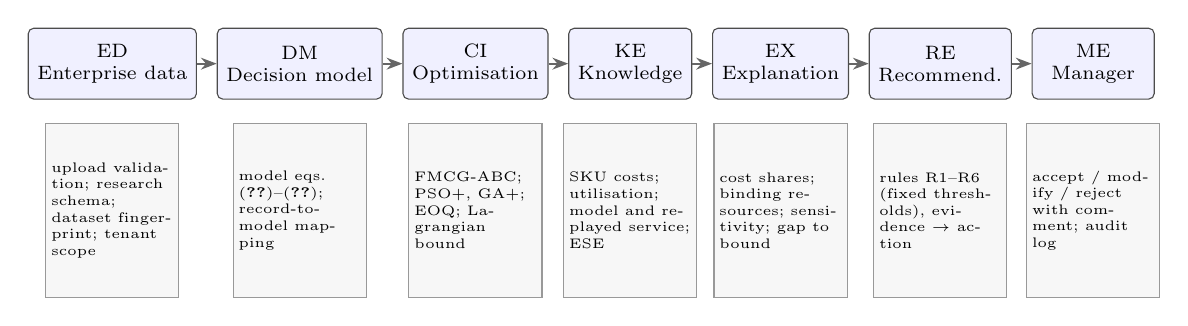
\begin{tikzpicture}[
  stage/.style={draw=black!70, rounded corners=2pt, fill=blue!6, minimum width=1.55cm, minimum height=0.9cm, align=center, font=\scriptsize},
  impl/.style={draw=black!40, fill=black!3, text width=1.55cm, minimum height=2.2cm, align=left, font=\tiny, inner sep=2pt},
  arr/.style={-{Stealth[length=2mm]}, thick, black!60}]
\node[stage] (ed) {ED\\Enterprise data};
\node[stage, right=0.25cm of ed] (dm) {DM\\Decision model};
\node[stage, right=0.25cm of dm] (ci) {CI\\Optimisation};
\node[stage, right=0.25cm of ci] (ke) {KE\\Knowledge};
\node[stage, right=0.25cm of ke] (ex) {EX\\Explanation};
\node[stage, right=0.25cm of ex] (re) {RE\\Recommend.};
\node[stage, right=0.25cm of re] (me) {ME\\Manager};
\foreach \a/\b in {ed/dm,dm/ci,ci/ke,ke/ex,ex/re,re/me} \draw[arr] (\a) -- (\b);
\node[impl, below=0.3cm of ed] {upload validation; research schema; dataset fingerprint; tenant scope};
\node[impl, below=0.3cm of dm] {model eqs.\ (\ref{eq:sdlt})--(\ref{eq:bounds}); record-to-model mapping};
\node[impl, below=0.3cm of ci] {FMCG-ABC; PSO+, GA+; EOQ; Lagrangian bound};
\node[impl, below=0.3cm of ke] {SKU costs; utilisation; model and replayed service; ESE};
\node[impl, below=0.3cm of ex] {cost shares; binding resources; sensitivity; gap to bound};
\node[impl, below=0.3cm of re] {rules R1--R6 (fixed thresholds), evidence $\to$ action};
\node[impl, below=0.3cm of me] {accept / modify / reject with comment; audit log};
\end{tikzpicture}}
\caption{EIDSF stages (top) and their implementation in the Inventory Intelligence Dashboard (bottom).}\label{fig:framework}
\end{figure}

\paragraph{Enterprise data} The IID accepts operational inventory files (stock, demand, cost, lead time, supplier and warehouse attributes) through a validating upload service that rejects files it cannot interpret and reports every derived field. A separate research-dataset schema validates the thesis data format (SKU, segment, annual demand, demand standard deviation, unit, ordering, holding and shortage costs, lead time and unit volume) without storing or altering values, records a content fingerprint, and requires the units of each field to be confirmed before the data can enter the model (Table~\ref{tab:dict}). All data are scoped to an organisation (tenant).

\begin{table}[!htbp]
\centering\footnotesize
\caption{Thesis dataset (30 SKUs): fields, model symbols and status in the IID research schema.}\label{tab:dict}
\begin{tabular}{p{0.26\linewidth}p{0.17\linewidth}p{0.47\linewidth}}
\toprule
Thesis field & Model symbol & Status \\
\midrule
SKU\_ID, Segment & $i$, class & identifiers \\
Annual\_Demand\_Dbar & $D_i$ ($d_i=D_i/365$) & units per year \\
Demand\_StdDev\_Sigma & $\sigma_{d,i}$ & period (daily or annual) to be confirmed \\
Unit\_Cost\_c & $p^{reg}_i$ & currency to be confirmed; no discount data \\
Ordering\_Cost\_s & $K_i$ & per order \\
Holding\_Cost\_h & $h_i$ & basis (absolute or rate) to be confirmed \\
Shortage\_Cost\_pi & $c_{s,i}$ & basis (per unit or per unit-time) to be confirmed \\
Lead\_Time\_L & $L_i$ & unit to be confirmed; $\sigma_{L,i}$ not recorded \\
Unit\_Volume\_v & $v_i$ & unit to be confirmed; warehouse assignment not recorded \\
\bottomrule
\end{tabular}
\end{table}

\paragraph{Decision model and computational intelligence} The model of Section~\ref{sec:model} and the methods of Section~\ref{sec:abc} are implemented in one Python package (\texttt{eidsf}) that is used both by the experiments in this paper and by an authenticated DSS service. The service maps the organisation's current inventory records to the model (the mapping assumptions are returned with every result), runs the selected method, and computes the Lagrangian bound for the same instance (by default for portfolios of up to 1{,}000 SKUs; for larger ones the bound takes several minutes and is computed on request). Figure~\ref{fig:iid} shows the resulting view.

\paragraph{Knowledge extraction, explanation and recommendation} For every SKU and for the portfolio, the artifact reports the policy, its cost components and their shares, resource utilisation, model-implied and (where a replay is available) realised service, the expected shortage exposure, the gap to the lower bound, and the recommendation rules that fired with their evidence (Section~\ref{sec:artifact}).

\paragraph{Managerial evaluation} Recommendations enter a decision workflow in which a manager accepts, modifies or rejects each one; modifications and rejections require a comment, and each decision is stored with the dataset identity, a snapshot of the recommendation and the user, so that the decision can later be traced to the evidence on which it was based. The system does not place orders.

%% ============================================================================
\section{Decision model}\label{sec:model}

\subsection{Assumptions and notation}
We consider $N$ SKUs indexed by $i$, assigned to warehouses $w=1,\dots,W$ ($I_w$ is the set of SKUs in warehouse $w$), and a planning year of 365 days. SKU $i$ has mean daily demand $d_i$ with standard deviation $\sigma_{d,i}$, annual demand $D_i=365d_i$, mean lead time $L_i$ (days) with standard deviation $\sigma_{L,i}$, ordering cost $K_i$ per order, holding cost $h_i$ per unit and year, shortage cost $c_{s,i}$ per unit short, regular price $p^{reg}_i$, discounted price $p^{disc}_i<p^{reg}_i$ for orders of at least $q^{disc}_i$ units (all-units discount), unit volume $v_i$, and target cycle service level $\alpha_i\ge 0.5$. $B$ is the procurement budget, defined below, and $Cap_w$ the capacity of warehouse $w$. Demand and lead time are independent, lead-time demand is approximated as normal for the service and expected-shortage calculations, and shortages are backordered. The decision variables are the order quantity $Q_i$ and the safety stock $SS_i$; the reorder point is derived as $ROP_i=d_iL_i+SS_i$.

\subsection{Costs}
The standard deviation of lead-time demand is
\begin{equation}\label{eq:sdlt}
\sdlt=\sqrt{L_i\sigma_{d,i}^2+d_i^2\sigma_{L,i}^2},
\end{equation}
and the standardised safety stock is $z_i=SS_i/\sdlt$, with model-implied cycle service level
\begin{equation}\label{eq:cslmodel}
CSL^{\mathrm{model}}_i=\Phi(z_i).
\end{equation}
With $\mathcal{L}(z)=\phi(z)-z\,[1-\Phi(z)]$ the standard normal loss function, the expected shortage per cycle is $ES_i=\sdlt\,\mathcal{L}(z_i)$ and, with $D_i/Q_i$ cycles per year, the annual cost is
\begin{equation}\label{eq:tc}
TC(Q,SS)=\sum_{i=1}^N\Big[\underbrace{K_i\frac{D_i}{Q_i}}_{C_{o,i}}+\underbrace{h_i\Big(\frac{Q_i}{2}+SS_i\Big)}_{C_{h,i}}+\underbrace{c_{s,i}\frac{D_i}{Q_i}\sdlt\,\mathcal{L}(z_i)}_{C_{s,i}}+\underbrace{D_i\,p_i(Q_i)}_{C_{p,i}}\Big],
\end{equation}
where $p_i(Q_i)=p^{disc}_i$ if $Q_i\ge q^{disc}_i$ and $p^{reg}_i$ otherwise. Because $C_{p,i}\ge D_i\min(p^{reg}_i,p^{disc}_i)$, we also report the \emph{controllable cost} $\Cctrl=TC-C_0$ with the constant $C_0=\sum_i D_i\min(p^{reg}_i,p^{disc}_i)$; all relative gaps in this paper are computed on $\Cctrl$, because ratios of $TC$, which is dominated by purchasing, make large differences in ordering, holding and shortage look negligible.

\subsection{Constraints and complete model}
\begin{align}
\min_{Q,SS}\quad & TC(Q,SS) \nonumber\\
\text{s.t.}\quad & \textstyle\sum_{i} p_i(Q_i)\,Q_i \le B, \label{eq:budget}\\
& \textstyle\sum_{i\in I_w} v_i\,(Q_i/2+SS_i)\le Cap_w,\qquad w=1,\dots,W, \label{eq:wh}\\
& \Phi(SS_i/\sdlt)\ge\alpha_i\iff SS_i\ge z_{\alpha_i}\sdlt,\quad z_{\alpha_i}=\Phi^{-1}(\alpha_i), \label{eq:service}\\
& Q^{\min}_i\le Q_i\le Q^{\max}_i,\qquad 0\le SS_i\le SS^{\max}_i. \label{eq:bounds}
\end{align}
Constraint (\ref{eq:budget}) limits the purchase value of one replenishment batch of every SKU, that is, the procurement commitment if all SKUs were replenished at the same time; it is the budget formulation of the thesis and uses the active price, so that taking a discount changes both the purchasing cost and the commitment. It is not the average capital tied up in stock, $\sum_i p_i(Q_i)(Q_i/2+SS_i)$, under which safety stock would also consume budget. Both forms are used in practice and they bind differently; the convexity argument and the bound carry over to the average-investment form, which is also linear within each price regime. The main results use (\ref{eq:budget}); the comparison is repeated with the average-investment form in Section~\ref{sec:res-variants}. Likewise, the continuous-review assumption is relaxed in a variant that subtracts the expected review-period undershoot $u_i$ from the protection, $z_i=(SS_i-u_i)/\sdlt$, which shifts the service bound to $SS_i\ge z_{\alpha_i}\sdlt+u_i$ and leaves Proposition~\ref{prop:convex} intact. The warehouse constraint (\ref{eq:wh}) limits average stored volume; a peak-volume version would replace $Q_i/2$ by $Q_i$. Two corrections relative to earlier versions of this model are worth stating: the shortage cost uses the expected shortage quantity (loss function) rather than the stockout probability times demand, and the expected shortage exposure used in the artifact is $ESE_i=(D_i/Q_i)\,ES_i/D_i=ES_i/Q_i$, the expected fraction of annual demand that is short, rather than the dimensionally inconsistent $ES_i/D_i$.

\subsection{Structure and a certified lower bound}

The structure of the model rests on one inequality for the standard normal distribution. Let $\bar\Phi=1-\Phi$ and let $R(z)=\bar\Phi(z)/\phi(z)$ be Mills' ratio, so that $\mathcal{L}(z)=\phi(z)\,[1-zR(z)]$.

\begin{lemma}\label{lem:mills}
For every $z\ge0$, $2\mathcal{L}(z)\phi(z)-\bar\Phi(z)^2>0$.
\end{lemma}
\begin{proof}
Dividing by $\phi(z)^2>0$, the claim is $2(1-zR)-R^2>0$, that is $R^2+2zR-2<0$. Because $R>0$, this is equivalent to $R(z)<b(z):=\sqrt{z^2+2}-z$, the positive root of $r^2+2zr-2$. Mills' ratio satisfies $R'(z)=zR(z)-1$, and
\[
b'(z)-\big(zb(z)-1\big)=\frac{z\,\big(z\sqrt{z^2+2}-z^2-1\big)}{\sqrt{z^2+2}}\le0\quad(z\ge0),
\]
with equality only at $z=0$, because $(z^2+1)^2-z^2(z^2+2)=1>0$ gives $z\sqrt{z^2+2}<z^2+1$. Hence $\Delta=b-R$ satisfies $\Delta'-z\Delta=b'-zb+1\le0$, so $e^{-z^2/2}\Delta(z)$ is non-increasing on $[0,\infty)$. Since $0<R(z)\le R(0)$ and $0<b(z)\le\sqrt2$, $e^{-z^2/2}\Delta(z)\to0$ as $z\to\infty$; a non-increasing function with limit zero is non-negative, and it is strictly positive because its derivative is negative on $(0,\infty)$. Thus $\Delta(z)>0$ for all $z\ge0$.
\end{proof}

\begin{proposition}\label{prop:convex}
For a fixed price regime of each SKU (that is, restricting $Q_i$ to $Q_i<q^{disc}_i$ or to $Q_i\ge q^{disc}_i$), model (\ref{eq:tc})--(\ref{eq:bounds}) is a convex program, provided that $\sigma_{DLT,i}>0$, $c_{s,i}>0$, $D_i>0$ and $\alpha_i\in[0.5,1)$ for all $i$. The same holds for the average-investment budget and for the review-period variant, in which $z_i=(SS_i-u_i)/\sigma_{DLT,i}$ is an affine shift.
\end{proposition}
\begin{proof}
Within a regime, $C_{o,i}$ is convex in $Q_i>0$, $C_{h,i}$ is linear, $C_{p,i}$ is constant, and the constraints are linear. For the shortage term $g(Q,S)=c\,\mathcal{L}(S/\sigma)/Q$ with $c=c_{s}D\sigma>0$, using $\mathcal{L}'(z)=-\bar\Phi(z)$ and $\mathcal{L}''(z)=\phi(z)$,
\begin{gather*}
g_{QQ}=\frac{2c\mathcal{L}}{Q^3},\qquad g_{SS}=\frac{c\,\phi}{\sigma^2Q},\qquad g_{QS}=\frac{c\,\bar\Phi}{\sigma Q^2},\\
\det\nabla^2g=\frac{c^2}{\sigma^2Q^4}\Big(2\mathcal{L}(z)\phi(z)-\bar\Phi(z)^2\Big),
\end{gather*}
evaluated at $z=S/\sigma$. The diagonal entries are positive because $\mathcal{L}>0$ and $\phi>0$. The service constraint (\ref{eq:service}) with $\alpha_i\ge0.5$ restricts the feasible set to $z\ge z_{\alpha_i}\ge0$, where the determinant is positive by Lemma~\ref{lem:mills}. Hence $\nabla^2g$ is positive definite on the convex feasible set and $g$ is convex there. (If $\sigma_{DLT,i}=0$ the shortage term vanishes and the claim holds trivially; the argument uses $\alpha_i\ge0.5$ only to guarantee $z\ge0$, and for $z<0$ convexity is not claimed.) The proposition is analytic; the numerical checks of the Hessian in the test suite are a safeguard against implementation errors, not part of the proof.
\end{proof}

The derivatives and the determinant were also checked symbolically. Numerically, the bracket remains non-negative down to $z\approx-0.5506$, but we use and claim convexity only for $z\ge0$, which is all the model requires. The same argument covers the review-period variant of Section~\ref{sec:res-variants}, in which $z=(S-u)/\sigma$ is an affine function of $S$, and the average-investment budget, which is linear within a regime.

Quantity discounts therefore make the problem non-convex only through the choice among $2^N$ price-regime combinations. We relax the budget and warehouse constraints with multipliers $\lambda\ge0$ and $\mu\in\mathbb{R}^W_{\ge0}$:
\begin{multline}\label{eq:dual}
g(\lambda,\mu)=\sum_{i=1}^N\min_{(Q_i,SS_i)\in X_i}\Big[TC_i+\lambda p_i(Q_i)Q_i+\mu_{w(i)}v_i\big(\tfrac{Q_i}{2}+SS_i\big)\Big]\\
-\lambda B-\sum_w\mu_wCap_w,
\end{multline}
where $X_i$ collects (\ref{eq:service}) and (\ref{eq:bounds}). By weak duality, $g(\lambda,\mu)\le TC^*$ for every $\lambda,\mu\ge0$ \citep{Everett1963,Fisher1981}; this holds whether or not the primal problem is convex, provided each inner minimum is computed exactly, because an overestimated inner minimum could overstate the bound. The relaxation separates by SKU, and each SKU is solved for its two price regimes separately and the cheaper one kept, so the $2^N$ combinations never have to be enumerated. Within a regime, the inner objective is convex in $SS_i$ for fixed $Q_i$ ($g_{SS}>0$), and its first-order condition gives the closed form
\begin{equation}\label{eq:ssopt}
1-\Phi(z_i^*)=\frac{(h_i+\mu_{w(i)}v_i)\,Q_i}{c_{s,i}D_i},\qquad SS_i^*=\sdlt\cdot\mathrm{clip}\big(z_i^*,\,z_{\alpha_i},\,SS_i^{\max}/\sdlt\big),
\end{equation}
where clipping to the bounds is exact for a one-dimensional convex function. Because the inner objective is jointly convex in $(Q_i,SS_i)$ on the regime (Proposition~\ref{prop:convex}) and the bounds on $SS_i$ do not depend on $Q_i$, its partial minimum over $SS_i$ is a convex function of $Q_i$; it is therefore unimodal in $\log Q_i$ as well, and a golden-section search on $\log Q_i$ (120 iterations, after which the interval is reduced by a factor of about $10^{-25}$), compared with the two end points of the regime, returns the regime minimum up to floating-point precision. We maximise $g$ by coordinate ascent over $(\lambda,\mu)$; ascent need not reach the dual optimum, but every point it visits is a valid bound. Without discounts the program is convex with linear constraints and a strictly feasible point, strong duality holds \citep{Boyd2004} and the bound is tight; with discounts it remains a valid lower bound but a duality gap can remain. In both cases the gap of any feasible policy to the bound is an upper bound on its true optimality gap, which the DSS reports with every recommendation. The multipliers at the best dual point are the sensitivities of the bound with respect to the resource limits; they equal the shadow prices of the optimal cost only in the convex case (and where the optimal value is differentiable), and with discounts they should be read as approximate indicators of where additional resources would pay off.

%% ============================================================================
\section{FMCG-ABC}\label{sec:abc}

\subsection{Search space and standard ABC}
All stochastic methods search $x\in[0,1]^{2N}$ that a common decoder maps to $(Q,SS)$, call the same evaluation function, and stop after the same number $E_{\max}$ of objective evaluations. In standard ABC \citep{Karaboga2007}, a colony of $2\cdot SN$ bees maintains $SN$ food sources (candidate policies). Each employed bee perturbs one randomly chosen dimension $k$ of its source $x_j$ towards or away from a random other source $x_r$, $v_{jk}=x_{jk}+\varphi_{jk}(x_{jk}-x_{rk})$ with $\varphi_{jk}\sim U(-1,1)$, and keeps the better of $x_j$ and $v_j$ (greedy selection); onlooker bees repeat this for sources chosen with probability increasing in quality; a source not improved for \emph{limit} trials is replaced by a random scout. We use rank-proportional onlooker selection (scale-free and identical in all variants), $SN=50$, limit $=120$, and $E_{\max}=50{,}000$.

\subsection{FMCG-specific adaptations}
FMCG-ABC adds three groups of adaptations, which the ablation in Section~\ref{sec:results} evaluates cumulatively:
\begin{description}
\item[A2.] \emph{EOQ-informed initialisation.} Half of the initial sources are placed around the EOQ policy, $Q_{ij}=Q^{EOQ}_i(1+\epsilon_{ij})$ with $\epsilon_{ij}\sim U(-0.2,0.2)$ and $SS_{ij}=z_{\alpha_i}\sdlt(1+U(0,0.2))$; the other half are uniform random.
\item[A3.] \emph{Inventory-specific constraint adaptation.} (i) The service constraint (\ref{eq:service}) is encoded as a lower bound of $SS_i$, so every decoded policy meets it. (ii) A repair restores the coupling constraints: if (\ref{eq:budget}) or (\ref{eq:wh}) is violated, $Q$ and $SS$ are moved along the segment towards their lower bounds, $(Q,SS)(t)=(Q^{\min},z_\alpha\sigma_{DLT})+t\,[(Q,SS)-(Q^{\min},z_\alpha\sigma_{DLT})]$, and $t\in[0,1]$ is chosen by 30 bisection steps that keep the lower end of the bracket feasible; the repaired policy is written back into the source (Lamarckian repair). Without discounts, resource use is increasing in $t$ and the bisection returns the largest feasible $t$. With all-units discounts, budget use can increase when an order quantity falls below its discount threshold, so the feasible set of $t$ need not be an interval; the bisection then still returns a feasible point, but not necessarily the largest feasible $t$. If the lower-bound policy ($t=0$) is itself infeasible, no feasible policy exists and the method reports infeasibility. (iii) Sources are ranked feasibility-first \citep{Deb2000}: feasible before infeasible, feasible by $TC$, infeasible by normalised violation. Without A3, constraints are handled by the normalised quadratic penalty $F=TC+\rho\sum_j\tilde V_j^2$, with $\tilde V$ the violations scaled by the service requirement, $B$ and $Cap_w$ and $\rho=10^3\,TC(\text{EOQ})$, fixed before the experiments.
\item[A4.] \emph{Inventory-specific perturbation (full FMCG-ABC).} Order quantities are decoded on a logarithmic scale, so that ABC moves are multiplicative and comparable across SKUs whose quantities differ by orders of magnitude, and each dimension is perturbed with probability $MR=0.1$ (at least one), in the spirit of \citet{Akay2012}, instead of exactly one.
\end{description}
In every variant the reported solution is the best feasible policy evaluated during the run; if none is feasible, the least-violating policy is retained only as a diagnostic and reported as infeasible. Algorithm~\ref{alg:abc} summarises FMCG-ABC.

\begin{algorithm}[!htbp]
\caption{FMCG-ABC}\label{alg:abc}
\footnotesize
\begin{algorithmic}[1]
\Require instance data, $SN$, limit, $E_{\max}$, $MR$, seed
\State initialise $SN$ sources: 50\% around $(Q^{EOQ},z_\alpha\sigma_{DLT})$, 50\% uniform in the encoded box
\State decode (log-$Q$, service-as-bound), repair, write back, evaluate; set trial counters to 0
\While{evaluations $<E_{\max}$}
  \For{each source $j$ (employed) and then $SN$ sources drawn by rank (onlookers)}
    \State $v\gets x_j$; for each dimension $k$ with probability $MR$: $v_k\gets x_{jk}+\varphi(x_{jk}-x_{rk})$
    \State decode, repair, write back, evaluate $v$; if $v$ ranks before $x_j$ (feasibility first) then $x_j\gets v$, trial$_j\gets0$ else trial$_j\gets$ trial$_j+1$
  \EndFor
  \State if $\max_j$ trial$_j\ge$ limit: replace that source by a uniform random scout
  \State record the best feasible policy found so far
\EndWhile
\State \Return best feasible policy (or a diagnostic, flagged infeasible)
\end{algorithmic}
\end{algorithm}

\subsection{Comparators}
\emph{EOQ with static safety stock} uses the all-units-discount EOQ procedure per SKU and $SS_i=z_{\alpha_i}\sdlt$, ignoring the coupling constraints (its feasibility is reported). \emph{GA} is a real-coded GA with binary tournament selection, simulated binary crossover ($p_c=0.9$, $\eta_c=15$), polynomial mutation ($p_m=1/(2N)$, $\eta_m=20$), elitism of two and population 100 \citep{DebAgrawal1995}. \emph{PSO} is global-best PSO with constriction coefficients ($w=0.7298$, $c_1=c_2=1.49618$, velocity clamp 0.2) and swarm 100 \citep{ClercKennedy2002}. GA, PSO and ABC (A1) use the penalty approach. To separate the effect of the search engine from that of the inventory adaptations, \emph{GA+} and \emph{PSO+} receive exactly the A3 adaptations (EOQ initialisation, service-as-bound, repair and feasibility-first ranking). All parameters were fixed before the experiments and are listed in Table~\ref{tab:config}.

\begin{table}[!htbp]
\centering\footnotesize
\caption{Method configuration (fixed before the experiments).}\label{tab:config}
\begin{tabular}{p{0.2\linewidth}p{0.72\linewidth}}
\toprule
All methods & $E_{\max}=50{,}000$ evaluations (10{,}000 on 6-SKU instances); 30 runs (main instance) with seeds 1--30; NumPy PCG64 generator; same decoder, evaluation and best-solution rule \\
ABC variants & colony 100 ($SN=50$), limit 120, rank-proportional onlookers; A1 random init., penalty, linear $Q$, one dimension per move; A2 +EOQ init.\ (50\%, $\delta=0.2$); A3 +service bound, repair, feasibility-first; A4 (FMCG-ABC) +log-$Q$, $MR=0.1$ \\
GA / GA+ & population 100, tournament 2, SBX $p_c=0.9$, $\eta_c=15$, polynomial mutation $p_m=1/(2N)$, $\eta_m=20$, elitism 2 \\
PSO / PSO+ & swarm 100, $w=0.7298$, $c_1=c_2=1.49618$, $|v|\le0.2$ \\
Penalty & $F=TC+\rho\sum_j\tilde V_j^2$, $\rho=10^3\,TC(\text{EOQ})$ (A1, A2, GA, PSO) \\
Software & Python 3.12, NumPy 2.1, SciPy 1.14, pandas 2.2 \\
\bottomrule
\end{tabular}
\end{table}

%% ============================================================================
\section{Evaluation design}\label{sec:design}

\subsection{Synthetic FMCG portfolios}
Because the evaluation requires many controlled instances, known data-generating processes and a holdout period, the experiments use a documented generator (Table~\ref{tab:gen}). Daily demand is Gamma distributed with a coefficient of variation between 0.15 and 0.75, deliberately not normal, so that the normal approximation of the model is tested out of sample. The first 730 days calibrate $d_i$ and $\sigma_{d,i}$ (sample mean and standard deviation); the last 270 days are held out for policy replay. Service targets follow an ABC classification by annual demand value. The discount threshold lies above the EOQ, so that the discount creates a genuine order-size trade-off. The budget and warehouse capacities are set to a fraction $\tau_B$, $\tau_C$ of what the EOQ policy would use, so that the coupling constraints bind. All instances are generated from fixed seeds and labelled synthetic throughout; no result in this paper is based on real company data.

\begin{table}[!htbp]
\centering\footnotesize
\caption{Synthetic portfolio generator (per SKU unless stated).}\label{tab:gen}
\begin{tabular}{p{0.33\linewidth}p{0.6\linewidth}}
\toprule
Mean daily demand & $\mathrm{LogNormal}(\ln40,1)$, clipped to [2, 600] units/day \\
Daily demand series (1000 days) & $\mathrm{Gamma}$ with mean $d_i$ and $CV_i\sim U(0.15,0.75)$ \\
Lead time & $L_i\sim U\{3,\dots,21\}$ days; $\sigma_{L,i}=L_i\cdot U(0.1,0.3)$ \\
Regular price; discount & $p^{reg}_i\sim U(80,1500)$; rate $U(0.02,0.08)$; $q^{disc}_i=U(1,2)\times Q^{EOQ}_i$ \\
Holding, ordering, shortage cost & $h_i=U(0.18,0.30)\,p^{reg}_i$; $K_i\sim U(1500,6000)$; $c_{s,i}=U(0.25,0.80)\,p^{reg}_i$ \\
Unit volume; warehouse & $v_i\sim U(0.0008,0.012)\,\mathrm{m}^3$; uniform over $W=2$ warehouses \\
Service target & 0.98 / 0.95 / 0.90 for the top 20\% / next 30\% / last 50\% by annual demand value \\
Bounds & $Q^{\min}_i=\max(1,d_i)$, $Q^{\max}_i=6Q^{EOQ}_i$, $SS^{\max}_i=4\sigma_{DLT,i}$ \\
Budget; capacity & $B=\tau_B\sum_ip_i(Q^{EOQ}_i)Q^{EOQ}_i$; $Cap_w=\tau_C\sum_{i\in I_w}v_i(Q^{EOQ}_i/2+SS_i)$ \\
Calibration / holdout & days 1--730 / 731--1000 \\
\bottomrule
\end{tabular}
\end{table}

\subsection{Experiments}
\begin{description}
\item[E1 Main comparison.] One 50-SKU instance (seed 2026, $\tau_B=0.75$, $\tau_C=0.80$); EOQ and eight stochastic methods (GA, PSO, ABC, A2, A3, FMCG-ABC, GA+, PSO+), 30 runs each.
\item[E2 Certified gap, convex case.] The E1 instance without discounts ($p^{disc}=p^{reg}$), for which the Lagrangian bound is tight; six methods, 10 runs.
\item[E3 Exact optimum with discounts.] Five 6-SKU instances ($\tau_B=0.70$, $\tau_C=0.75$) whose reference optimum is obtained by enumerating all $2^6$ price regimes, each a convex program (Proposition~\ref{prop:convex}) solved by sequential quadratic programming on a scaled formulation from six starting points, and certified afterwards by per-regime Lagrangian bounds (S1); six methods, 10 runs each.
\item[E4 Robustness.] Five further 50-SKU instances at tight ($\tau=0.60$) and loose ($\tau=0.90$) resources; ABC, FMCG-ABC, GA+, PSO+, 3 runs each.
\item[E5 Scalability.] $N\in\{25,50,75,100\}$, one instance per size, 10 runs, fixed $E_{\max}$.
\item[E6 Sensitivity.] The E1 instance with $\sigma_d\times\{0.8,1.2\}$, $\alpha_i\{-0.03,+0.01\}$, $B\times\{0.9,1.1\}$ and $Cap_w\times\{0.9,1.1\}$, re-optimised with FMCG-ABC (5 runs).
\item[E7 Out-of-sample replay.] The median run of each method in E1 and the EOQ policy are replayed on the 270-day holdout.
\end{description}
Six extension experiments were added in revision to address the limits of E1--E7 (\texttt{python -m eidsf.extend}). \emph{X1} gives PSO+ and GA+ the number of evaluations they can perform in the time FMCG-ABC needs for 50{,}000 (equal wall-clock time; seeds 1--10). \emph{X2} repeats E5 on three generated instances per size (seeds $3000+N$, $3100+N$, $3200+N$; five runs each). \emph{X3} and \emph{X4} add runs to E4 (five per instance) and E6 (ten per scenario). \emph{X5} replaces the budget by the average capital tied up in stock, $\sum_ip_i(Q_i)(Q_i/2+SS_i)\le B$; \emph{X6} builds the expected daily-review undershoot $u_i=(\sigma_{d,i}^2+d_i^2)/(2d_i)$ into the model by measuring protection as $SS_i-u_i$ in the service constraint and the shortage cost (both with ten runs per method and the Lagrangian bound, which extends to both variants).
Three supplementary analyses were added after the main run to check the references and to explain observed results; they did not change any E1--E7 result. \emph{S1} certifies the E3 references by computing, for every price regime, the Lagrangian bound of the convex regime problem and taking the minimum over regimes. \emph{S2} recomputes the E1 bound with the budget or the capacities scaled by 0.9 and 1.1 and compares the change with the first-order estimate from the multipliers. \emph{S3} replays the median FMCG-ABC policy under normal instead of Gamma demand and with an allowance for daily-review undershoot (Section~\ref{sec:replay}).

\subsection{Policy replay}
A fixed policy $(Q_i, ROP_i)$ is replayed against the observed holdout demand with daily review and backorders. Each day, arriving orders first clear backorders; demand is served from stock and the unmet part is backordered; if the inventory position (on hand minus backorders plus on order) is at or below $ROP_i$, $k\,Q_i$ units are ordered with $k$ the smallest integer that lifts the position above $ROP_i$; the lead time is drawn from $\max(1,\mathrm{round}(N(L_i,\sigma_{L,i}^2)))$ and the order is usable from the start of day $t+LT+1$. After a 30-day warm-up we record the realised cycle service level (share of replenishment cycles without a stockout day), the fill rate ($1-$ backordered units / demand), shortage units and annualised costs. Replications (30) differ only in lead-time draws.

\subsection{Metrics and statistics}
For each method we report the number of feasible runs, and over feasible runs the mean, standard deviation, median and interquartile range of $\Cctrl$ and the median gap to the best known feasible solution (BKS) or to the certified or exact optimum. Gap $=100\,(TC-TC^*)/(TC^*-C_0)$. The sensitivity of the policy cost to a parameter change $\theta\to\theta+\Delta$ (with re-optimisation) is
\begin{equation}\label{eq:si}
SI_\theta=\frac{TC(\theta+\Delta)-TC(\theta)}{TC(\theta)},
\end{equation}
reported on $TC$ and, as $SI^{ctrl}$, on $\Cctrl$. Runs of different methods use the same integer seeds but not the same random numbers, because each method consumes its generator stream differently; on one instance they are therefore independent samples, not pairs. We compare FMCG-ABC with each other method by the two-sided Mann--Whitney U test \citep{MannWhitney1947} with Holm correction \citep{Holm1979}, report a percentile-bootstrap 95\% confidence interval of the difference of medians (both groups resampled independently, 5{,}000 resamples) and the Vargha--Delaney effect size $A_{12}$, the probability that a randomly chosen FMCG-ABC run is cheaper than a randomly chosen run of the comparator \citep{VarghaDelaney2000}, and apply a Kruskal--Wallis test \citep{KruskalWallis1952} across methods. Paired tests over problem instances, as recommended by \citet{Derrac2011} for comparisons across many problems, would require more instances than our design contains. Statistical tests are only applied to methods feasible in all runs; an infeasible policy is never compared on cost.

\subsection{Reproducibility}
All experiments are run by one command (\texttt{python -m eidsf.study}); every table and figure in Section~\ref{sec:results} is generated from the stored outputs by \texttt{python -m eidsf.report}, and the run configuration (seeds, software versions, rule thresholds and runtime) is written next to the results. The supplementary analyses, the extensions and the statistical comparison are run by the modules \texttt{eidsf.supplement}, \texttt{eidsf.extend} and \texttt{eidsf.stats\_unpaired} of the same package. Before submission, 134 numbers stated in this paper were checked automatically against the stored result files, and a subset of 57 values covering every experiment type was re-computed in a fresh environment built from the pinned library versions; all matched exactly. The model equations, the bound, the methods, the replay, the artifact and the price, budget and repair behaviour immediately below, at and above discount thresholds are covered by automated tests, several of which compare against values computed by hand from the equations above.

%% ============================================================================
\section{Results}\label{sec:results}
%% RESULTS-START (written after the study run; every number checked against generated/values.json and the CSV files)
%% All numbers in this file were checked against backend/experiments/results/eidsf/2026-10-18/
%% (e1_summary.csv, e1_stats.csv, e2_certified.csv, e3_small_exact.csv, e4_robustness.csv,
%% e5_scalability.csv, e6_sensitivity.csv, e7_replay.csv, reference_bounds.csv, run_config.json).
All results in this section are from synthetic instances (Section~\ref{sec:design}). The complete study (920 optimisation runs, bounds, exact references and replays) took 68 minutes on two CPU cores, and the extension experiments (370 runs) a further 77 minutes.

\subsection{Feasibility and cost (E1)}\label{sec:res-e1}
Table~\ref{tab:e1} reports the main comparison. The EOQ policy with static safety stock needs 133\% of the budget and 125\% of the capacity of the more constrained warehouse; its controllable cost (16.0 million) is therefore not attainable. Imposing the shared resources roughly doubles the controllable cost of the best feasible policies, which is the cost of coupling that independent EOQ planning hides.

The three generic penalty-based methods rarely returned an admissible policy: PSO in none of 30 runs, standard ABC in one and GA in nine, and the feasible GA and ABC policies cost more than twice the best known solution (BKS). Their returned solutions violated the constraints only slightly in normalised terms (median normalised violation 0.1\% for GA, 0.7\% for ABC and 20\% for PSO), which is the typical outcome of a quadratic penalty that trades a small violation for a large cost reduction. All four constraint-adapted methods were feasible in every run. Among them FMCG-ABC had the lowest median controllable cost (34.10 million, interquartile range 2.52), ahead of PSO+ (40.23) and GA+ (40.30); A3, which shares the constraint handling of FMCG-ABC but not its log-scale multi-dimensional move, reached 54.21. The best known feasible solution (29.71 million) was found by FMCG-ABC (seed 15); the best GA+ and PSO+ runs reached 31.93 and 32.01. Figure~\ref{fig:box} shows the run distributions.

\begin{table}[!htbp]
\centering
\footnotesize
\caption{Main comparison on the synthetic 50-SKU portfolio ($N=50$, $\tau_B=0.75$, $\tau_C=0.80$; 30 independent runs per stochastic method, $E_{\max}=50{,}000$ objective evaluations). Cost statistics are over feasible runs only, on the controllable-cost scale (millions of currency units).}\label{tab:e1}
\resizebox{\linewidth}{!}{%
\begin{tabular}{lrrrrrrrrr}
\toprule
Method & Feasible & $U_B$ (\%) & $\max_w U_w$ (\%) & Median & IQR & Mean & SD & $\Delta_{\mathrm{BKS}}$ (\%) & Time (s) \\
\midrule
EOQ + static SS & 0/1 & 133.3 & 125.0 & 15.98 & 0.00 & 15.98 & 0.00 & -- & 0.0 \\
GA & 9/30 & 94.9 & 99.8 & 78.52 & 7.25 & 78.89 & 4.83 & 164.3 & 2.1 \\
PSO & 0/30 & 85.6 & 98.9 & -- & -- & -- & -- & -- & 0.4 \\
ABC (A1) & 1/30 & 93.5 & 99.7 & 80.51 & 0.00 & 80.51 & -- & 171.0 & 14.2 \\
FMCG-ABC (A4) & 30/30 & 99.9 & 99.9 & 34.10 & 2.52 & 34.31 & 2.23 & 14.8 & 31.6 \\
GA+ & 30/30 & 99.9 & 99.9 & 40.30 & 4.51 & 42.18 & 5.05 & 35.7 & 3.3 \\
PSO+ & 30/30 & 100.0 & 99.9 & 40.23 & 2.09 & 39.17 & 4.45 & 35.4 & 1.7 \\
\bottomrule
\end{tabular}}
\par\smallskip\parbox{0.95\linewidth}{\scriptsize $U_B$, $U_w$: median budget and highest warehouse utilisation of the returned policy (values above 100 indicate violation). $\Delta_{\mathrm{BKS}}$: median gap to the best known feasible solution over all runs. Controllable cost $= TC - \sum_i D_i\min(p_i^{reg},p_i^{disc})$ (a constant shift). Lagrangian lower bound: 25.02; best known feasible: 29.71.}
\end{table}


\begin{figure}[!htbp]
\centering
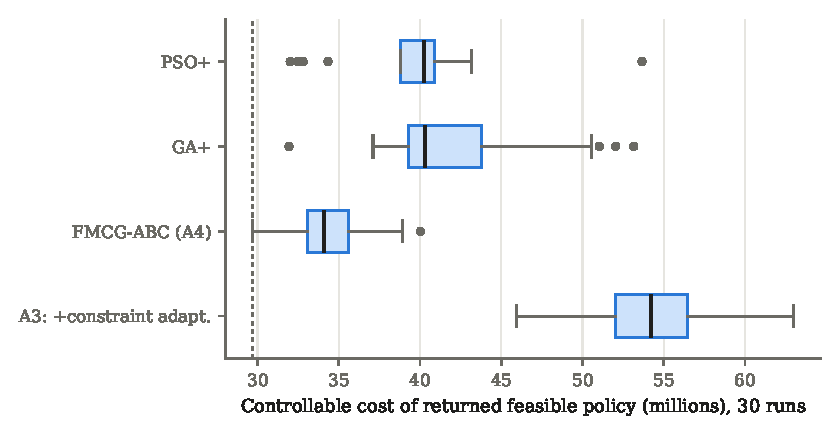
\includegraphics[width=0.78\linewidth]{generated/fig_cost_box.pdf}
\caption{Distribution over 30 runs of the controllable cost of the returned feasible policy, main instance. Dashed line: best known feasible solution.}\label{fig:box}
\end{figure}

Table~\ref{tab:stats} reports the statistical comparison. Across the four methods that were feasible in all runs, the Kruskal--Wallis test rejects equal distributions ($H=83.9$, $p<10^{-4}$). The medians of FMCG-ABC were lower than those of A3, GA+ and PSO+ by 20.11, 6.20 and 6.12 million, with bootstrap confidence intervals that exclude zero; all three Mann--Whitney tests remain significant after Holm correction ($p<10^{-4}$). A randomly chosen FMCG-ABC run was cheaper than a randomly chosen run of A3, GA+ and PSO+ with probability $A_{12}=1.00$, 0.95 and 0.81: the advantage over PSO+ is clear but not uniform. Methods that were infeasible in some runs were not tested on cost.

\begin{table}[!htbp]
\centering
\footnotesize
\caption{Comparison of FMCG-ABC with each method feasible in all runs on the main instance (two-sided Mann--Whitney U test on controllable cost, Holm correction; runs of different methods are independent).}\label{tab:stats}
\resizebox{\linewidth}{!}{%
\begin{tabular}{lrrrrrr}
\toprule
Comparison & $n$ & $U$ & $p$ & $p_{\mathrm{Holm}}$ & Diff.\ of medians [95\% CI] & $A_{12}$ \\
\midrule
FMCG-ABC vs A3 & 30/30 & 0 & $<10^{-4}$ & $<10^{-4}$ & -20.11 [-21.57, -18.79] & 1.00 \\
FMCG-ABC vs GA+ & 30/30 & 43 & $<10^{-4}$ & $<10^{-4}$ & -6.20 [-7.80, -5.28] & 0.95 \\
FMCG-ABC vs PSO+ & 30/30 & 172 & $<10^{-4}$ & $<10^{-4}$ & -6.12 [-6.93, -4.84] & 0.81 \\
\bottomrule
\end{tabular}}
\par\smallskip\parbox{0.95\linewidth}{\scriptsize Difference of medians: FMCG-ABC minus comparator, millions; negative favours FMCG-ABC; CI: percentile bootstrap of both groups independently (5000 resamples). $A_{12}$: probability that a randomly chosen FMCG-ABC run is cheaper than a randomly chosen comparator run (Vargha--Delaney). Kruskal--Wallis test across the four methods: $H=83.9$, $p<10^{-4}$.}
\end{table}


\subsection{How far from optimal? (E1--E3)}\label{sec:res-gap}
The Lagrangian lower bound for the main instance is 25.02 million; the BKS is 18.7\% above it and the FMCG-ABC median 36.3\% above it. Because the instance has quantity discounts, the bound is not tight, and these percentages are upper bounds on the true gaps rather than estimates. E2 and E3 measure the gaps exactly (Table~\ref{tab:exact}).

\begin{table}[!htbp]
\centering
\footnotesize
\caption{Gaps to a certified optimum: (a) main instance without quantity discounts (convex; optimum certified by the Lagrangian dual, duality gap 0.0000\%); (b) five 6-SKU instances with discounts (optimum by enumerating all $2^6$ price regimes).}\label{tab:exact}
\resizebox{\linewidth}{!}{%
\begin{tabular}{lrrrrrr}
\toprule
Method & \multicolumn{3}{c}{(a) $N=50$, convex} & \multicolumn{3}{c}{(b) $N=6$, discounts} \\ \cmidrule(lr){2-4}\cmidrule(lr){5-7} & Feas. (\%) & Median gap & Max gap & Feas. (\%) & Median gap & Max gap \\
\midrule
GA & 10 & 49.96 & 49.96 & 100 & 11.58 & 48.12 \\
PSO & 0 & -- & -- & 100 & 47.29 & 131.26 \\
ABC (A1) & 0 & -- & -- & 100 & 17.50 & 63.85 \\
FMCG-ABC (A4) & 100 & 0.10 & 0.11 & 100 & 7.85 & 47.30 \\
GA+ & 100 & 0.10 & 0.15 & 100 & 7.66 & 47.39 \\
PSO+ & 100 & 0.17 & 0.22 & 100 & 7.61 & 47.29 \\
\bottomrule
\end{tabular}}
\par\smallskip\parbox{0.95\linewidth}{\scriptsize Gap $=(TC-TC^{*})/(TC^{*}-C_0)\times100$ on feasible runs, $C_0=\sum_i D_i\min(p^{reg}_i,p^{disc}_i)$. (a) 10 runs per method, $E_{\max}$ as in Table~\ref{tab:e1}; (b) 10 runs per instance, $E_{\max}=10{,}000$.}
\end{table}


Without discounts (E2) the bound and the best dual-recovered primal policy coincide (duality gap $10^{-6}$\%), so the optimum is certified. The three adapted methods then came within 0.10\% (FMCG-ABC, GA+) and 0.17\% (PSO+) of the optimum in median, while penalty-based PSO and ABC returned no feasible policy and GA one policy 50\% above the optimum. On the five small discounted instances (E3) all methods were feasible, and the three adapted methods had almost identical median gaps (PSO+ 7.6\%, GA+ 7.7\%, FMCG-ABC 7.9\%); FMCG-ABC had the lowest per-instance median on three of the five instances. Their worst runs were 47\% above the optimum, and the generic methods were further away. To find the cause, we solved each instance separately for every price-regime combination and re-ran the adapted methods (10 seeds each): 135 of 150 runs ended in a suboptimal combination of regimes, 104 of the 106 runs with a gap above 5\% did so, and within the regime they selected, the runs were a median 0.15\% from that regime's optimum. Together with E2, this locates the hardness of the model in the discrete choice of price regimes rather than in the continuous part, which the adapted methods solve almost exactly.\footnote{The exact references of E3 were first computed with an unscaled sequential quadratic programming solver; because some heuristic runs then beat the reported ``optimum'', which is impossible, the references were recomputed with a scaled formulation from six starting points. After the correction no run beats the reference (smallest gap 0.04\%), and the per-regime Lagrangian bounds of S1 certify every corrected reference to within $2\times10^{-6}$\% of controllable cost, so they are optimal to numerical precision. The heuristic runs did not depend on the reference and were not repeated.}

\subsection{Which adaptation matters? (ablation)}\label{sec:res-ablation}
Table~\ref{tab:ablation} adds the adaptations one at a time. EOQ-informed initialisation (A2) raised the number of feasible runs from 1 to 21 of 30 and lowered the median feasible cost from 80.5 to 60.9 million, but still left infeasible runs, because a penalised search can drift away from a feasible start. The inventory-specific constraint handling (A3: service-as-bound, repair and feasibility-first ranking) made every run feasible and lowered the median to 54.2 million. The log-scale multi-dimensional move (A4) produced the largest single improvement, to 34.1 million. The same constraint handling also made GA and PSO competitive (GA+, PSO+), so the constraint adaptations are not specific to ABC; what distinguished FMCG-ABC from the adapted GA and PSO in E1 is the combination with the perturbation scheme.

\begin{table}[!htbp]
\centering
\footnotesize
\caption{Ablation of the FMCG-specific adaptations (main instance).}\label{tab:ablation}
\resizebox{\linewidth}{!}{%
\begin{tabular}{lrrrrrr}
\toprule
Configuration & Feasible & Median & $\Delta_{\mathrm{BKS}}$ (\%) & Med. viol. (\%) & Realised CSL (\%) & Fill (\%) \\
\midrule
ABC (A1) & 1/30 & 80.51 & 171.0 & 0.74 & 97.8 & 99.59 \\
A2: +EOQ init. & 21/30 & 60.93 & 105.1 & 0.00 & 96.3 & 99.61 \\
A3: +constraint adapt. & 30/30 & 54.21 & 82.5 & 0.00 & 94.7 & 99.68 \\
FMCG-ABC (A4) & 30/30 & 34.10 & 14.8 & 0.00 & 92.9 & 99.34 \\
\bottomrule
\end{tabular}}
\par\smallskip\parbox{0.95\linewidth}{\scriptsize Median cost over feasible runs (millions; -- if none). Median violation: normalised aggregate violation of the returned solution. Realised CSL and fill rate: holdout replay of the median run (Table~\ref{tab:replay}); for A1 the median run is infeasible, so its replay describes an inadmissible policy.}
\end{table}


\subsection{Convergence}
Figure~\ref{fig:conv} shows the best feasible cost against the number of evaluations (median and interquartile band over 30 runs). PSO+ improved fastest initially and led until about 10{,}000 evaluations, after which it stagnated near 40 million; FMCG-ABC kept improving until the end of the budget. The curves are still decreasing at 50{,}000 evaluations, so all methods would benefit from a larger budget, and the ranking at a much smaller budget would differ.

\begin{figure}[!htbp]
\centering
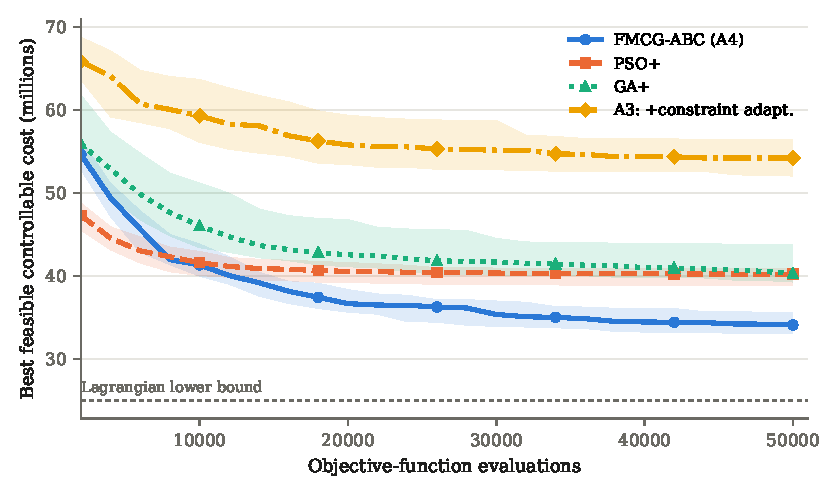
\includegraphics[width=0.85\linewidth]{generated/fig_convergence.pdf}
\caption{Best feasible controllable cost versus objective evaluations on the main instance (line: median of 30 runs; band: interquartile range). Dashed: Lagrangian lower bound.}\label{fig:conv}
\end{figure}

\subsection{Equal wall-clock time (X1)}\label{sec:res-time}
Because our ABC implementation evaluates and repairs one candidate at a time, whereas GA and PSO evaluate whole populations in vectorised form, FMCG-ABC needed about 32 seconds per run on the main instance against 2 seconds for PSO+ and 3 seconds for GA+. To check whether the ranking depends on the equal-evaluation criterion, we gave PSO+ and GA+ the number of evaluations they can perform in the time FMCG-ABC needs for 50{,}000 (952{,}752 and 478{,}667 evaluations; Table~\ref{tab:x1}). With 10 to 19 times more evaluations, and in practice slightly more time than FMCG-ABC, both remained more expensive: median controllable cost 40.24 (PSO+) and 38.35 million (GA+) against 34.00 million, The difference to GA+ is significant (Mann--Whitney, Holm-adjusted $p<0.001$, $A_{12}=1.00$); the difference to PSO+ is not ($p=0.064$, $A_{12}=0.75$, and the confidence interval of the difference of medians, $[-7.59,+1.65]$ million, includes zero). With ten independent runs per method, we therefore conclude that FMCG-ABC was not worse than PSO+ at equal time and better than GA+, not that its advantage over PSO+ survives equal time; the additional evaluations did not move PSO+ and GA+ in median away from the region where they stagnate (Figure~\ref{fig:conv}).

\begin{table}[!htbp]
\centering
\footnotesize
\caption{Equal wall-clock time (X1): adapted GA and PSO receive the number of evaluations they can perform in the mean time FMCG-ABC needs for 50{,}000 evaluations; seeds 1--10, main instance.}\label{tab:x1}
\resizebox{\linewidth}{!}{%
\begin{tabular}{lrrrrrrrr}
\toprule
Comparator & Evaluations & Feasible & FMCG-ABC & Comparator & Time (s) & Diff.\ of medians, 95\% CI & $p_{\mathrm{Holm}}$ & $A_{12}$ \\
\midrule
PSO+ & 952,752 & 10/10 & 34.00 & 40.24 & 32 / 46 & [-7.59, +1.65] & 0.0640 & 0.75 \\
GA+ & 478,667 & 10/10 & 34.00 & 38.35 & 32 / 44 & [-6.62, -3.50] & 0.0004 & 1.00 \\
\bottomrule
\end{tabular}}
\par\smallskip\parbox{0.95\linewidth}{\scriptsize Median controllable cost (millions); FMCG-ABC values are its E1 runs with the same seeds. Time: mean seconds per run, FMCG-ABC / comparator. Runs are independent samples (10 per method): two-sided Mann--Whitney U test with Holm correction, Vargha--Delaney $A_{12}$, bootstrap 95\% CI of the difference of medians.}
\end{table}


\subsection{Robustness and scalability (E4, E5, X2, X3)}\label{sec:res-robust}
Across five further 50-SKU instances with five runs each (Table~\ref{tab:robust}), FMCG-ABC had the lowest median gap to the best solution found for each instance at tight resources (4.7\% vs.\ 10.3\% for PSO+ and 13.4\% for GA+) and at loose resources (5.5\% vs.\ 14.1\% and 19.1\%). It attained the best solution in 4 of 25 runs at tight resources, but at loose resources PSO+ did so more often (3 vs.\ 1 of 25 runs), so the median advantage does not mean that FMCG-ABC finds the best policy most often. Standard ABC was never feasible at tight resources and feasible in 5 of 25 runs at loose resources.

\begin{table}[!htbp]
\centering
\footnotesize
\caption{Robustness across five independently generated 50-SKU instances at tight ($\tau=0.60$) and loose ($\tau=0.90$) coupling constraints (5 runs per instance and method; E4 extended by X3).}\label{tab:robust}
\resizebox{\linewidth}{!}{%
\begin{tabular}{lrrrrrr}
\toprule
Method & \multicolumn{3}{c}{$\tau=0.60$} & \multicolumn{3}{c}{$\tau=0.90$} \\ \cmidrule(lr){2-4}\cmidrule(lr){5-7} & Feas. (\%) & Med. $\Delta_{\mathrm{best}}$ (\%) & Wins & Feas. (\%) & Med. $\Delta_{\mathrm{best}}$ (\%) & Wins \\
\midrule
ABC (A1) & 0 & -- & 0 & 20 & 124.8 & 0 \\
FMCG-ABC (A4) & 100 & 4.7 & 4 & 100 & 5.5 & 1 \\
GA+ & 100 & 13.4 & 0 & 100 & 19.1 & 1 \\
PSO+ & 100 & 10.3 & 1 & 100 & 14.1 & 3 \\
\bottomrule
\end{tabular}}
\par\smallskip\parbox{0.95\linewidth}{\scriptsize $\Delta_{\mathrm{best}}$: gap to the best feasible cost found for that instance by any method; Wins: runs attaining it (out of 25).}
\end{table}


For scalability we used three generated instances per size and five runs per instance (Table~\ref{tab:scal}, Figure~\ref{fig:scal}). FMCG-ABC had the lowest median gap for $N=50$, 75 and 100 (4.2\%, 5.3\% and 4.9\%), but not for $N=25$, where PSO+ was ahead (8.3\% vs.\ 10.9\%). Standard ABC was feasible only for $N=25$. An earlier single-instance version of this experiment (E5, 10 runs) had ranked GA+ first for $N=100$; the three-instance results show that this ranking was specific to that instance, which is why we report the extended design. Runtime grows with $N$ for all methods, and FMCG-ABC remained the slowest per evaluation.

\begin{table}[!htbp]
\centering
\footnotesize
\caption{Scalability: median gap to the best feasible solution of each instance, over three generated instances per size and 5 runs each (E5 extended by X2), and mean runtime per run.}\label{tab:scal}
\resizebox{\linewidth}{!}{%
\begin{tabular}{lrrrrrrrr}
\toprule
Method & \multicolumn{2}{c}{$N=25$} & \multicolumn{2}{c}{$N=50$} & \multicolumn{2}{c}{$N=75$} & \multicolumn{2}{c}{$N=100$} \\ \cmidrule(lr){2-3}\cmidrule(lr){4-5}\cmidrule(lr){6-7}\cmidrule(lr){8-9} & $\Delta_{\mathrm{best}}$ (\%) & s & $\Delta_{\mathrm{best}}$ (\%) & s & $\Delta_{\mathrm{best}}$ (\%) & s & $\Delta_{\mathrm{best}}$ (\%) & s \\
\midrule
ABC (A1) & 60.9 & 13 & infeas. & 14 & infeas. & 14 & infeas. & 14 \\
FMCG-ABC (A4) & 10.9 & 39 & 4.2 & 48 & 5.3 & 51 & 4.9 & 53 \\
GA+ & 12.7 & 4 & 13.0 & 4 & 14.2 & 5 & 11.6 & 6 \\
PSO+ & 8.3 & 2 & 9.1 & 2 & 7.0 & 3 & 7.8 & 3 \\
\bottomrule
\end{tabular}}
\par\smallskip\parbox{0.95\linewidth}{\scriptsize Runtimes were measured with two runs in parallel on two cores and include repair; they are comparable within a column only.}
\end{table}


\begin{figure}[!htbp]
\centering
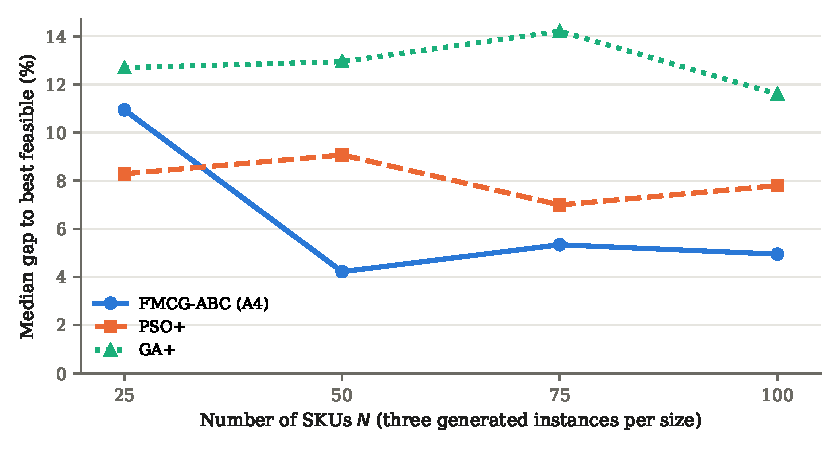
\includegraphics[width=0.78\linewidth]{generated/fig_scalability.pdf}
\caption{Median gap to the best feasible solution per instance size (three instances per size, five runs each).}\label{fig:scal}
\end{figure}

\subsection{Sensitivity (E6, X4)}\label{sec:res-sens}
Table~\ref{tab:sens} reports the re-optimised FMCG-ABC policy cost for one-at-a-time parameter changes, with ten runs per scenario and the sensitivity index of equation~(\ref{eq:si}) on controllable cost. On total cost every change is below 0.5\%, because purchasing dominates $TC$. On controllable cost, a 10\% tighter warehouse capacity raised the cost by 18.5\%, a 10\% tighter budget by 14.4\% and a one-point higher service target by 11.4\%, while a 10\% larger budget lowered it by 16.8\%; a 10\% larger capacity and a three-point lower service target lowered it by about 5\%. Demand variability moved it by $-3.2\%$ ($\sigma_d\times0.8$) and $+7.0\%$ ($\sigma_d\times1.2$). The resource effects exceed the run-to-run variability of FMCG-ABC (interquartile range 7\% of the median) and agree in sign with the change of the lower bound (Section~\ref{sec:artifact}); the demand-variability effects are of the order of that variability. On this portfolio, the binding resources and the service targets drive the cost of the policy more than demand variability does.

\begin{table}[!htbp]
\centering
\footnotesize
\caption{Sensitivity of the re-optimised FMCG-ABC policy cost to model parameters (10 runs per scenario; E6 extended by X4).}\label{tab:sens}
\begin{tabular}{lrrrr}
\toprule
Scenario & Feas. (\%) & Median ctrl. cost & IQR & $SI^{ctrl}$ (\%) \\
\midrule
$\sigma_d\times0.8$ & 100 & 33.01 & [31.73, 34.63] & -3.2 \\
$\sigma_d\times1.2$ & 100 & 36.48 & [34.93, 37.91] & +7.0 \\
$\alpha_i-0.03$ & 100 & 32.52 & [32.04, 33.17] & -4.6 \\
$\alpha_i+0.01$ & 100 & 37.99 & [35.70, 38.92] & +11.4 \\
$B\times0.9$ & 100 & 39.00 & [37.65, 40.33] & +14.4 \\
$B\times1.1$ & 100 & 28.39 & [28.14, 29.67] & -16.8 \\
$Cap_w\times0.9$ & 100 & 40.41 & [39.50, 41.17] & +18.5 \\
$Cap_w\times1.1$ & 100 & 32.44 & [32.11, 32.94] & -4.9 \\
\bottomrule
\end{tabular}
\par\smallskip\parbox{0.95\linewidth}{\scriptsize $SI^{ctrl}$: change of the median controllable cost relative to the median of the 30 E1 runs (34.10 million), eq.~(\ref{eq:si}). Base run-to-run IQR: 2.52 million (7.4\%).}
\end{table}


\subsection{Out-of-sample service (E7)}\label{sec:replay}
Table~\ref{tab:replay} reports the replay of each method's median policy on the 270-day holdout. All feasible policies met their targets on average in the model (mean model-implied CSL 95.0--96.4\% against a mean target of 93.1\%), but realised CSL was lower: 92.9\% for FMCG-ABC, 92.3\% for PSO+, 94.8\% for GA+ and 94.7\% for A3, with 25 to 28 of the 50 SKUs below their individual targets. Fill rates remained above 99.3\%. The EOQ policy realised 90.5\% with 38 SKUs below target. Cycle service level and fill rate measure different things: a stockout that is cleared within a day hardly affects the fill rate but makes the whole cycle a failure, so a high portfolio fill rate does not imply that every SKU meets its cycle-service target.

To explain the shortfall we replayed the median FMCG-ABC policy under variants (S3, Table~\ref{tab:s3}). Replacing the Gamma holdout by normal demand with the calibrated mean and standard deviation did not remove the shortfall (realised CSL 91.7\%, 28 SKUs below target), so the non-normality of demand is not its main cause. Adding to each reorder point the expected undershoot of daily review, $(\sigma_{d,i}^2+d_i^2)/(2d_i)$, which the continuous-review model ignores, raised the realised CSL to 95.3\% and reduced the SKUs below target from 27 to 17, at 2{,}562 additional units of safety stock and 0.54 million of additional holding cost. The corrected policy, however, needs 105.4\% of the capacity of the second warehouse and is therefore infeasible: the allowance must be built into the model and re-optimised, not added afterwards (Section~\ref{sec:res-variants}). The 17 remaining shortfalls indicate further sources that we did not isolate, such as integer lead times and the short holdout. Policies with less safety stock above the service requirement are the most exposed: FMCG-ABC and PSO+, whose mean model-implied CSL (95.0\% and 95.5\%) is closer to the targets than that of GA+ and A3 (96.3\% and 96.4\%), show the larger shortfall. Model feasibility is therefore necessary but not sufficient for service, which is why the artifact reports realised service next to the model-implied value and rule R1 fires when they diverge.

\begin{table}[!htbp]
\centering\footnotesize
\caption{Replay diagnostic for the median FMCG-ABC policy (S3; 30 lead-time replications each).}\label{tab:s3}
\resizebox{\linewidth}{!}{%
\begin{tabular}{lrrr}
\toprule
Variant & Realised CSL (\%) & Fill rate (\%) & SKUs $<\alpha_i$ \\
\midrule
(a) Gamma holdout (as in Table~\ref{tab:replay}) & 92.9 & 99.34 & 27 \\
(b) Normal demand, calibrated mean and s.d. & 91.7 & 99.45 & 28 \\
(c) Gamma holdout + undershoot allowance & 95.3 & 99.61 & 17 \\
(d) Normal demand + undershoot allowance & 95.1 & 99.71 & 14 \\
\bottomrule
\end{tabular}}
\par\smallskip\parbox{0.95\linewidth}{\scriptsize Allowance $(\sigma_{d,i}^2+d_i^2)/(2d_i)$ added to $SS_i$; variants (c) and (d) exceed the capacity of warehouse 2 (105.4\%) and are diagnostics, not admissible policies.}
\end{table}

\begin{table}[!htbp]
\centering
\footnotesize
\caption{Out-of-sample replay of the median run of each method on the 270-day holdout demand (30 lead-time replications; daily review; backorders).}\label{tab:replay}
\resizebox{\linewidth}{!}{%
\begin{tabular}{lrrrrrrr}
\toprule
Method & Feasible & Model CSL & Realised CSL [95\% CI] & Fill rate & Short. units/yr & SKUs $<\alpha_i$ & Ctrl. cost \\
\midrule
EOQ + static SS & no & 93.1 & 90.5 [90.2, 90.9] & 99.48 & 7,996 & 38 & 17.47 \\
GA & no & 97.6 & 97.3 [97.2, 97.4] & 99.31 & 10,572 & 11 & 28.31 \\
PSO & no & 87.0 & 79.4 [79.2, 79.6] & 83.05 & 259,384 & 15 & 162.42 \\
ABC (A1) & no & 96.7 & 97.8 [97.7, 97.9] & 99.59 & 6,264 & 17 & 25.99 \\
FMCG-ABC (A4) & yes & 95.0 & 92.9 [92.6, 93.1] & 99.34 & 10,052 & 27 & 19.09 \\
GA+ & yes & 96.3 & 94.8 [94.6, 95.0] & 99.62 & 5,782 & 25 & 17.04 \\
PSO+ & yes & 95.5 & 92.3 [92.0, 92.6] & 99.48 & 7,943 & 28 & 17.21 \\
\bottomrule
\end{tabular}}
\par\smallskip\parbox{0.95\linewidth}{\scriptsize Model CSL: mean of $\Phi(z_i)$ (eq.~\ref{eq:cslmodel}); mean target $\bar\alpha=93.1\%$. Realised controllable cost excludes purchasing (millions). Demand in the holdout is Gamma-distributed, not normal.}
\end{table}


\subsection{Model variants (X5, X6)}\label{sec:res-variants}
Table~\ref{tab:variants} repeats the main comparison under two variants of the model. With the budget defined as the average capital tied up in stock (X5), the budget is the only binding resource at the dual solution (warehouse multipliers zero); all three adapted methods remained feasible in every run and standard ABC in none, and FMCG-ABC again had the lowest median controllable cost (53.64 million, against 56.56 for GA+ and 63.22 for PSO+) and the smallest dispersion. The conclusions of the comparison therefore do not depend on which budget definition is adopted, although the cost levels do.

With the daily-review undershoot built into the service constraint and the shortage cost (X6), the re-optimised FMCG-ABC policy cost 35.42 million, 3.9\% more than under the continuous-review model, and raised the realised cycle service level on the holdout from 92.9\% to 96.8\%, with 9 instead of 27 SKUs below their targets; GA+ and PSO+ reached 96.5\% and 95.9\%. Unlike the post-hoc allowance of S3, these policies respect the warehouse capacities. Most of the out-of-sample service shortfall reported above is thus removed by modelling the review period, at a modest increase of controllable cost. The variant is not uniformly better: it assumes that the review period stays daily, uses an approximation of the expected undershoot, still leaves 9 SKUs below target, and costs 1.3 million more per year; whether that is worthwhile depends on how the firm values the avoided stockouts beyond the shortage cost already in the model. It is therefore offered to planners as an alternative policy with its cost and service consequences, not as a replacement.

\begin{table}[!htbp]
\centering
\footnotesize
\caption{Model variants on the main instance (10 runs per method): budget as average capital tied up in stock (X5) and daily-review undershoot inside the model (X6).}\label{tab:variants}
\resizebox{\linewidth}{!}{%
\begin{tabular}{llrrrrrr}
\toprule
Variant & Method & Feasible & Median ctrl. & IQR & Lower bound & Realised CSL (\%) & SKUs $<\alpha_i$ \\
\midrule
Average-investment budget & ABC (A1) & 0/10 & -- & -- & 37.10 & -- & -- \\
 & FMCG-ABC (A4) & 10/10 & 53.64 & 1.29 &  & -- & -- \\
 & GA+ & 10/10 & 56.56 & 8.62 &  & -- & -- \\
 & PSO+ & 10/10 & 63.22 & 8.94 &  & -- & -- \\
Daily-review model & FMCG-ABC (A4) & 10/10 & 35.42 & 3.73 & 25.63 & 96.8 & 9 \\
 & GA+ & 10/10 & 42.99 & 2.44 &  & 96.5 & 9 \\
 & PSO+ & 10/10 & 41.26 & 0.88 &  & 95.9 & 16 \\
\bottomrule
\end{tabular}}
\par\smallskip\parbox{0.95\linewidth}{\scriptsize Millions of currency units. X5: $B=0.75\sum_ip_i(Q^{EOQ}_i)(Q^{EOQ}_i/2+SS_i)$. X6: offset $u_i=(\sigma_{d,i}^2+d_i^2)/(2d_i)$ in the service constraint and the shortage cost; realised service from the replay of the median run (main model, E1: FMCG-ABC 92.9\%, 27 SKUs below target).}
\end{table}



%% RESULTS-END

%% ============================================================================
\section{The decision artifact}\label{sec:artifact}
%% Numbers checked against artifact_fmcg_abc.json (first iteration), artifact_fmcg_abc_v2.json (second iteration), generated/tab_decomp.tex, tab_artifact.tex, tab_resources.tex.
This section demonstrates the decision artifact on the median FMCG-ABC policy of the main instance. The artifact is produced by the same code that the DSS service calls; in the DSS the replay-based fields are only available when a holdout replay has been run, and the rules that need them (R1, R6) are then reported as not evaluated rather than silently omitted.

\subsection{Economic explanation}
Table~\ref{tab:decomp} decomposes the model cost. Compared with the (infeasible) EOQ policy, the feasible FMCG-ABC policy orders smaller quantities for 33 of the 50 SKUs, which raises ordering cost by 82\% and lowers holding cost by 13\%; it takes the quantity discount for 17 SKUs, and purchasing cost rises by 1.3\% because the budget no longer allows the discount to be taken for every SKU where it pays. Total model cost is 1.4\% higher than the EOQ cost. Because the EOQ policy violates both limits, this is not a comparison of two admissible policies: it measures how much the unconstrained economic optimum understates the cost of a policy the organisation can actually finance and store (on the controllable scale, 16.0 against 34.1 million). At SKU level, holding is the largest controllable cost component for 30 SKUs and ordering for 20; shortage is never the largest. A manager therefore sees immediately that the policy is shaped by the trade-off between order frequency and stock investment under binding resources, not by shortage risk.

\begin{table}[!htbp]
\centering
\footnotesize
\caption{Model cost decomposition (millions per year): EOQ with static safety stock versus the median FMCG-ABC policy on the main instance.}\label{tab:decomp}
\begin{tabular}{lrrr}
\toprule
Component & EOQ + static SS & FMCG-ABC & Change (\%) \\
\midrule
Ordering & 2.93 & 5.32 & +81.5 \\
Holding & 11.37 & 9.94 & -12.5 \\
Shortage & 1.67 & 1.71 & +2.4 \\
Purchasing & 1,310.65 & 1,327.77 & +1.3 \\
Total & 1,326.62 & 1,344.75 & +1.4 \\
\bottomrule
\end{tabular}
\par\smallskip\parbox{0.95\linewidth}{\scriptsize The EOQ policy violates the coupling constraints (budget utilisation 133\%); FMCG-ABC budget utilisation 99.9\%, warehouse utilisation 95.2\%, 99.8\%.}
\end{table}


\subsection{Constraint and service explanation}
The policy uses 99.9\% of the budget and 95.2\% and 99.8\% of the two warehouses. Utilisation alone does not say which limits constrain the policy: the budget and the second warehouse are at their limits and have positive multipliers in the bound, whereas the first warehouse is highly used but its multiplier is zero (Table~\ref{tab:resources}). In the model, every SKU meets its service target, 15 of them exactly at the bound $SS_i=z_{\alpha_i}\sigma_{DLT,i}$. In the replay, 27 SKUs fall short of their target, the portfolio cycle service level is 92.9\% and the fill rate 99.3\%. The expected shortage exposure $ESE_i=ES_i/Q_i$ has a median of 0.31\% and a maximum of 1.8\% of annual demand.

\subsection{Recommendations and an SKU record}
Table~\ref{tab:rules} lists the recommendation rules. Their thresholds were fixed before the experiments and are stored with every artifact. Rules R1--R3 and R6 describe an SKU; R4 and R5 describe a shared resource and, after the first evaluation (below), are reported once per resource rather than in each SKU record.

\begin{table}[!htbp]
\centering\footnotesize
\caption{Recommendation rules (condition $\to$ evidence $\to$ action).}\label{tab:rules}
\begin{tabular}{@{}ll>{\raggedright\arraybackslash}p{0.3\linewidth}>{\raggedright\arraybackslash}p{0.15\linewidth}>{\raggedright\arraybackslash}p{0.27\linewidth}@{}}
\toprule
ID & Scope & Condition & Evidence & Action \\
\midrule
R1 & SKU & $CV_{d,i}>0.50$ and realised CSL $<\alpha_i$ & $CV$, realised CSL & increase protection, subject to budget and capacity \\
R2 & SKU & holding share of controllable cost $>0.50$ & $C_{h,i}/\Cctrl_i$ & review / reduce order quantity \\
R3 & SKU & $L_i>14$ days & $L_i$ & review supplier lead-time arrangement \\
R4 & resource & $U_w>0.95$; status from limit and multiplier $\mu_w$ & $U_w$, $\mu_w$ & redistribute or reduce inventory exposure \\
R5 & resource & $U_B>0.95$; status from limit and multiplier $\lambda$ & $U_B$, $\lambda$ & delay, split or reprioritise procurement \\
R6 & SKU & realised CSL $<\alpha_i-0.05$ and $ESE_i>0.01$ & CSL, $ESE_i$ & prioritise service protection \\
\bottomrule
\end{tabular}
\end{table}
 In the first design iteration, evaluated here, every rule was attached to SKU records, and on this policy the rules fired 155 times: R4 (warehouse) and R5 (budget) for all 50 SKUs, R2 (holding-dominated cost) for 27, R3 (long lead time) for 16, R1 (high variability with realised service below target) for 12, and R6 never. R4 and R5 carried no SKU-specific information, and R4 fired for every SKU of the first warehouse although that warehouse does not constrain the policy (see below). In the second iteration, which the DSS now implements, the SKU records contain only R1--R3 and R6 (55 firings on this policy), and the resources are reported once (Table~\ref{tab:resources}) with one of four statuses: \emph{constraining} (at the limit, utilisation $\ge99.5\%$, with a positive multiplier), \emph{high utilisation, not constraining} (above the threshold with a zero multiplier), \emph{high utilisation, marginal value not computed} (when no bound was computed), and \emph{not constraining}. Table~\ref{tab:artifact} shows the record of the SKU with the most rules fired. Its order quantity exceeds the EOQ (1{,}496 vs.\ 943 units) because ordering at least the discount threshold earns the lower price; holding is 85\% of its controllable cost, its lead time is 20 days, its demand is highly variable ($CV=0.70$), and its realised service (0.949) is below its target (0.98) although the model-implied value meets it. The record states each of these facts with the number behind it and the action it suggests, and leaves the trade-off between them to the manager: R1 suggests more protection, R2 a smaller order quantity, and the resource view adds that this SKU's warehouse is highly used but not constraining, whereas the budget is constraining, so additional protection must be financed by savings elsewhere in the portfolio.

\begin{table}[!htbp]
\centering
\footnotesize
\caption{SKU-level decision artifact generated by the system for one SKU of the main instance (median FMCG-ABC run). Every entry is computed from the policy, the model or the replay.}\label{tab:artifact}
\begin{tabular}{p{0.38\linewidth}p{0.55\linewidth}}
\toprule
Field & Value \\
\midrule
SKU & SIM-040 (warehouse 0) \\
Order quantity $Q_i$ (EOQ baseline) & 1,496 (943) \\
Safety stock $SS_i$ (baseline) & 1,030 (1,030) \\
Reorder point $ROP_i$ & 2,952 \\
Price paid / discount taken & 1,385.45 / yes \\
Ordering / holding / shortage cost & 51,947 / 723,971 / 73,236 \\
Purchasing cost & 48,606,996 \\
Primary controllable driver & holding (85\%) \\
Model / target / realised CSL & 0.980 / 0.98 / 0.949 \\
Realised fill rate & 0.9887 \\
Budget / warehouse utilisation & 99.9\% / 95.2\% \\
Rule R1 & CV 0.70 $>$ 0.5 and realised CSL 0.949 $<$ target 0.98 $\Rightarrow$ Increase protection inventory, subject to budget and warehouse capacity \\
Rule R2 & holding cost is 85\% of controllable cost $\Rightarrow$ Review / reduce the order quantity \\
Rule R3 & lead time 20 d $>$ 14 d $\Rightarrow$ Review the supplier lead-time arrangement \\
\bottomrule
\end{tabular}
\end{table}


\begin{table}[!htbp]
\centering
\footnotesize
\caption{Portfolio-level resource view of the median FMCG-ABC policy (second design iteration): utilisation, whether the limit is reached, and the multiplier of the Lagrangian bound.}\label{tab:resources}
\resizebox{\linewidth}{!}{%
\begin{tabular}{>{\raggedright\arraybackslash}p{0.17\linewidth}lrrr>{\raggedright\arraybackslash}p{0.17\linewidth}>{\raggedright\arraybackslash}p{0.42\linewidth}}
\toprule
Resource & Rule & Use (\%) & At limit & Multiplier & Status & Action \\
\midrule
Procurement budget & R5 & 99.9 & yes & 0.91 & constraining & Relieving this resource lowers cost; compare the marginal value with its price before requesting more. \\
Warehouse 0 & R4 & 95.2 & no & 0.00 & high use, not constraining & Monitor; at the current policy the limit does not raise cost. \\
Warehouse 1 & R4 & 99.8 & yes & 17,924.42 & constraining & Relieving this resource lowers cost; compare the marginal value with its price before requesting more space. \\
\bottomrule
\end{tabular}}
\par\smallskip\parbox{0.95\linewidth}{\scriptsize At limit: utilisation of at least 99.5\%. Multipliers from the best dual point of the E1 bound (budget: per currency unit; warehouses: per m$^3$); with quantity discounts they are sensitivities of the bound, not exact shadow prices of the optimal cost.}
\end{table}


\subsection{Fidelity and an observation for redesign}
By construction, every number in the artifact is recomputed from $(Q,SS)$ with the model of Section~\ref{sec:model} or taken from the replay, and the automated tests check that the cost components sum to the reported total and that each fired rule's evidence satisfies its condition (for example, that R3 fires only for lead times above the threshold). This gives explanation fidelity in the sense of a traceable recommendation $\to$ evidence $\to$ model-output chain; it does not establish that the explanations improve managers' decisions, which requires a user study. As an example of the chain, the R2 entry of Table~\ref{tab:artifact} traces to the holding cost $h_i(Q_i/2+SS_i)=723{,}971$ and the controllable cost $51{,}947+723{,}971+73{,}236=849{,}154$ of the same SKU, whose ratio 0.85 exceeds the threshold 0.50; a test recomputes this chain.

The artifact provides three kinds of explanation, and we claim no more for it. (i) \emph{Descriptive} explanations decompose the model cost of the recommended policy into its components and report utilisation and service (Tables~\ref{tab:decomp} and \ref{tab:artifact}). (ii) \emph{Model-based diagnostics} compare these quantities with thresholds fixed in advance (the rules) or with the dual information of the bound (the resource status). (iii) \emph{Counterfactual sensitivity} is obtained by re-optimising or recomputing the bound under a changed resource (Tables~\ref{tab:s2} and \ref{tab:sens}). None of them is causal: a rule states that a condition holds for the recommended policy, not that acting on it will improve the outcome, and the cost decomposition is an accounting identity of the model, not an attribution of realised costs.

The evaluation exposed a weakness of the first rule design, which led to the second iteration described above. Because an optimised policy exhausts the binding resources, the threshold rules R4 and R5 fire for every SKU in the warehouse or portfolio and carry no SKU-specific information, and high utilisation is not the same as a binding limit, nor a binding limit the same as a positive marginal value. The resources are therefore reported once at portfolio level, together with the value of relieving them, which the bound already provides. At the dual solution of the main instance, the budget multiplier is $\lambda=0.91$ and the warehouse multipliers are $\mu=(0,\;17{,}924)$ per m$^3$: the second warehouse binds in the relaxation, the first does not. Their first-order estimate for a 10\% change of the budget ($\pm3.73$ million) is close to the recomputed change of the bound ($+3.91$ million for a 10\% cut, $-3.22$ million for a 10\% increase; S2, Table~\ref{tab:s2}); for the capacities the response is asymmetric ($+1.23$ and $-0.12$ million against an estimate of $\pm0.49$ million), because the multipliers change once the second warehouse is relieved. These are changes of a lower bound, not of the cost of a particular policy, and with discounts the multipliers are only approximate shadow prices; they are nevertheless the kind of evidence a planner needs to decide whether to request more budget or space. The re-optimised FMCG-ABC policies move in the same direction (Table~\ref{tab:sens}).

\begin{table}[!htbp]
\centering\footnotesize
\caption{Change of the Lagrangian lower bound of the main instance when a resource is scaled (S2), against the first-order estimate from the multipliers (millions).}\label{tab:s2}
\begin{tabular}{lrrr}
\toprule
Scenario & Bound (controllable) & Change of bound & First-order estimate \\
\midrule
Base & 25.02 & -- & -- \\
$B\times0.9$ & 28.93 & $+3.91$ & $+3.73$ \\
$B\times1.1$ & 21.80 & $-3.22$ & $-3.73$ \\
$Cap_w\times0.9$ & 26.25 & $+1.23$ & $+0.49$ \\
$Cap_w\times1.1$ & 24.90 & $-0.12$ & $-0.49$ \\
\bottomrule
\end{tabular}
\end{table}

\subsection{The artifact in the decision support system}
Figure~\ref{fig:iid} shows the same artifact as the IID presents it, computed on the synthetic sample file distributed with the system (64 SKUs, no discount data, so the bound certifies the gap; values are illustrative and unrelated to the study instance). The planner selects a method and obtains the feasibility status, model cost, lower bound and certified gap (2.5\% here), budget and warehouse utilisation, the EOQ baseline, the count of fired rules with the rules that could not be evaluated without a replay, and one row per SKU with its policy, cost components, primary cost driver, model-implied service and the evidence and action of each fired rule; the mapping from inventory records to model parameters is stated below the table. Following the evaluation above, a second design iteration of the IID view reports binding resources once at portfolio level, with their shadow prices and the first-order saving from 10\% more of each resource; because the dashboard records hold no discount data, the model is convex there, the bound is tight, and the multipliers are the shadow prices of the optimal cost (where it is differentiable). Figure~\ref{fig:iid} shows why this matters: under the first rule design R5 would fire for all 64 SKUs because the policy uses 96.4\% of the budget, but the shadow price of the budget is zero, so the budget does not in fact constrain the policy; the view reports it as ``high utilisation, not constraining'' and every warehouse pool as not constraining. Recommendations are then accepted, modified or rejected in the decision workflow of Section~\ref{sec:framework}.

\begin{figure}[!htbp]
\centering
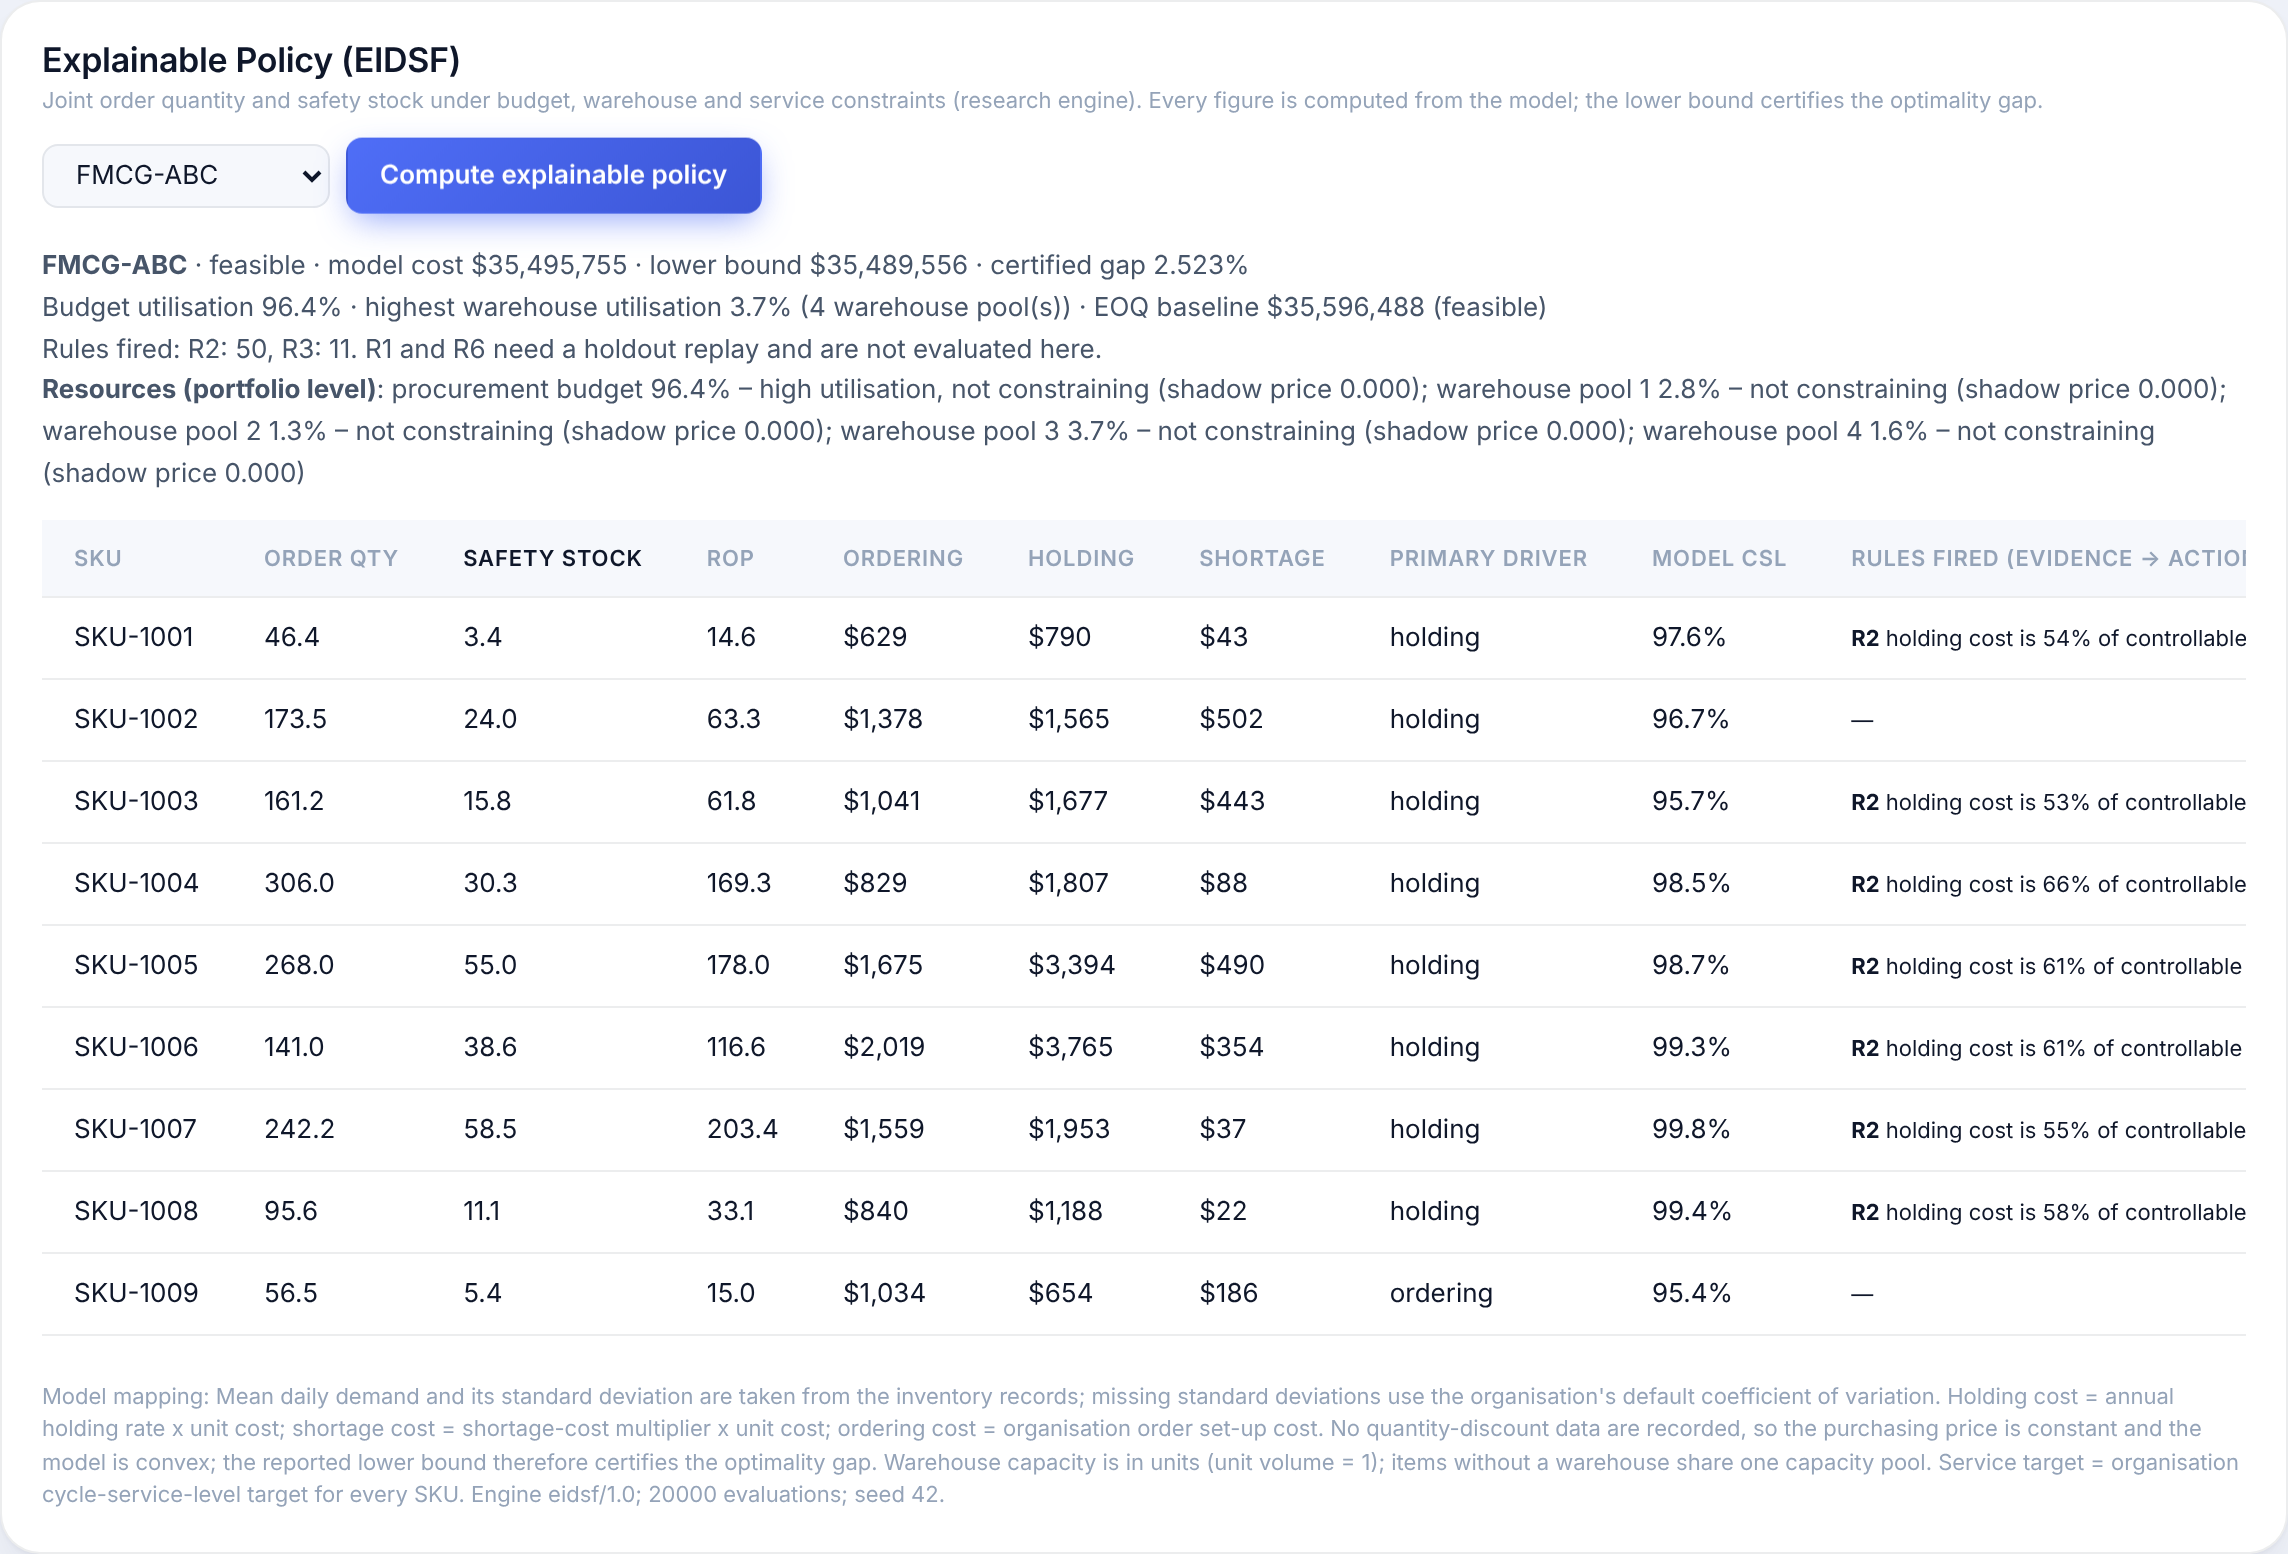
\includegraphics[width=\linewidth]{figures/fig_dashboard.png}
\caption{The explainable-policy view of the Inventory Intelligence Dashboard (FMCG-ABC, seed 42, 20{,}000 evaluations) on the synthetic sample file shipped with the system, after the second design iteration (portfolio-level resource status). The certified gap refers to the controllable cost. The rules column is truncated in the screenshot.}\label{fig:iid}
\end{figure}


%% ============================================================================
\ifrealdata
\section{Application to a distributor's portfolio}\label{sec:real}
% NOT INCLUDED unless \realdatatrue in main.tex.
% This section must only contain results produced by the code from the thesis' 30-SKU
% distributor dataset after its units (demand basis, sigma basis, lead-time unit, holding-cost
% basis, shortage-cost basis), budget, warehouse capacities, service targets and missing
% fields (lead-time variability, discounts, warehouse assignment) have been confirmed by
% the authors. No number may be copied from the thesis unless it is reproduced by the code.

\fi

%% ============================================================================
\section{Discussion}\label{sec:discussion}
\subsection{What the evidence shows, by dimension}
The findings concern different properties of the artifact, which should not be read as evidence for one another (Table~\ref{tab:dims}). Feasibility and solution quality are established on synthetic instances; computational efficiency is mixed; service reliability depends on the planning model more than on the search; managerial usefulness has not been tested.

\begin{table}[!htbp]
\centering\footnotesize
\caption{Findings by evaluation dimension.}\label{tab:dims}
\begin{tabular}{p{0.17\linewidth}p{0.47\linewidth}p{0.27\linewidth}}
\toprule
Dimension & Finding & Evidence and scope \\
\midrule
Feasibility & generic penalty methods rarely feasible under binding resources; all adapted methods always feasible & E1, E2, X2, X3, X5; synthetic \\
Solution quality & FMCG-ABC cheapest on the main instance and most instance groups; within 0.1\% of a certified optimum without discounts; about 8\% median and up to 47\% above the exact optimum with discounts for all adapted methods & E1--E3, X1--X5; certified or exact references where stated \\
Computational efficiency & 10--20 times slower per evaluation than vectorised GA+/PSO+; at equal time lowest median, significantly better than GA+ but not significantly better than PSO+ & E1, X1; one instance, one implementation \\
Service reliability & model-feasible policies miss individual targets for about half of the SKUs under daily review; the review-period variant reduces this to 9 of 50 at 3.9\% more cost & E7, S3, X6; synthetic holdout \\
Managerial usefulness & not evaluated & proposed study (Section~\ref{sec:limits}) \\
\bottomrule
\end{tabular}
\end{table}

The gap measures need the same care. Without discounts the bound is tight, so a gap to the bound is the true optimality gap. With discounts the bound can lie well below the optimum (the best known solution of the main instance is 18.7\% above it), so a large gap to the bound may reflect the bound rather than the policy; for the small instances, where the optimum is known, the methods themselves were about 8\% above it in the median. Planners should therefore read the reported gap as a guarantee (the policy is at most that far from optimal) and not as an estimate of the actual distance.

\subsection{Answers to the research questions}
\emph{RQ1.} The joint model represents the cost and service trade-offs of order quantity and safety stock with an expected-shortage cost and couples SKUs through the budget and the warehouses. Proposition~\ref{prop:convex} shows that its only source of non-convexity is the choice of price regimes, and the experiments confirm that this is where solution methods fail: without discounts, the adapted methods came within 0.1--0.2\% of a certified optimum, whereas on small discounted instances most runs selected a suboptimal combination of price regimes and stopped a median of about 8\%, and at worst 47\%, above the optimum.

\emph{RQ2.} The adaptations that matter most are inventory-specific constraint handling (service as a bound, repair, feasibility-first ranking), which turned a search that almost never returned a feasible policy into one that always did, and the log-scale multi-dimensional move, which reduced the median gap to the best known solution from 82\% to 15\%. EOQ-informed initialisation helped but did not, on its own, make the penalised search reliable. The constraint handling transfers to GA and PSO, so it is a property of the problem encoding rather than of the bee-colony metaphor.

\emph{RQ3.} FMCG-ABC returned the cheapest feasible policies on the main instance, with large and statistically significant differences at an equal evaluation budget. When the adapted GA and PSO received equal computing time, and therefore 10 to 19 times more evaluations, its median remained lowest; the difference was significant against GA+ but not against PSO+ with ten runs per method. It had the lowest median gap on the robustness instances, for portfolios of 50 to 100 SKUs over three instances per size, and under the average-investment budget. It was not the best method for 25-SKU portfolios, where PSO+ led, and on the small discounted instances the three adapted methods were practically tied. We therefore claim an advantage on these synthetic instance families, not general superiority. The more robust finding is negative and practical: generic penalty-based metaheuristics, as often used in inventory applications, returned inadmissible policies under binding resources.

\emph{RQ4.} The policies remained feasible under tighter and looser resources and for larger portfolios. The policy cost was most sensitive to the warehouse capacity, the budget and the service targets and little affected by demand variability. Out of sample, however, model-feasible policies missed individual service targets for about half of the SKUs, while fill rates stayed above 99\%. The diagnostic replay attributes most of the shortfall to the continuous-review assumption (undershoot of the reorder point under daily review) rather than to the normal approximation of demand, and building the review period into the model reduced the misses from 27 to 9 SKUs at 3.9\% higher controllable cost. This was a limitation of the planning model, not of the search, and it is the kind of discrepancy that an optimisation-only system would hide.

\emph{RQ5.} The artifact turns a policy into statements a planner can check: which cost component drives each SKU, which resources bind, how far the policy is from a lower bound, where model-implied and realised service diverge, and which rule fired on which evidence. The evaluation also showed that resource rules must be stated at portfolio level to remain informative.

\subsection{Implications for decision support design}
Three design principles generalise beyond inventory. First, \emph{feasibility is a first-class output}: a DSS that ranks candidate decisions by a penalised objective can recommend decisions that violate hard business limits by a small normalised amount but a large absolute one. Encoding the constraints the decision maker cannot negotiate as bounds or repairs, and reporting infeasibility rather than the least-bad candidate, prevented this. Second, \emph{a heuristic recommendation should carry a certificate}: a lower bound computed on the same instance turns ``the algorithm found this'' into ``this policy is at most $x$\% more expensive than any feasible policy'', which is an explanation of solution quality that managers and auditors can use, and in the convex case it is exact. Third, \emph{explanations must include what the model does not know}: reporting realised next to model-implied service exposed a systematic optimism of the planning model that an explanation of the optimisation alone would not reveal.

\subsection{Comparison with prior work}
Compared with the closest studies (Table~\ref{tab:position}), the improved ABC of \citet{Guo2025} addresses a single-item location--inventory problem with constant lead times and reports managerial insight through sensitivity analysis, and the decision support system of \citet{Long2023} optimises dynamic prices for a deteriorating product; neither treats several items competing for budget and storage, quantity discounts, or the quality of the returned solution. The multi-item studies closest in problem setting \citep{Pasandideh2013,Tan2024} treat discounts or a budget together with several items and compare metaheuristics, but report neither a bound on solution quality nor out-of-sample service, and neither embeds the result in an explanation layer. Classical multi-item results \citep{HadleyWhitin1963,RosenblattRothblum1990} provide the Lagrangian structure that our bound exploits but not the discounts, the service constraints or the decision support layer. Relative to the ABC literature \citep{Karaboga2008,Akay2012,Kaya2022}, our evidence is that, on this problem class, the problem-specific constraint handling matters more than the choice of swarm metaphor: the same handling made GA and PSO competitive. Relative to the explainable-AI literature for operational research \citep{DeBock2024,Coussement2024}, the artifact explains a decision rather than a prediction and attaches a bound on its quality, but, unlike the evaluation those authors call for, its effect on decision quality has not yet been measured.

\subsection{Managerial implications}
For FMCG planners, the results show that planning each SKU independently understates the controllable cost of a feasible policy by about half on the studied portfolio, that the budget and warehouse limits, not demand variability, drive the policy, and that service targets set in a continuous-review model should be checked against the review practice actually used. On the main instance, the multipliers of the bound put the value of an additional currency unit of procurement budget at about 0.9 currency units of annual controllable cost and identify the second warehouse as the binding space, which tells a planner where additional resources would pay off before any policy is changed. The DSS supports these checks without taking the decision: recommendations are accepted, modified or rejected by the planner, and the decision and its evidence are recorded.

\subsection{Limitations and future research}\label{sec:limits}
\emph{Data.} All results are synthetic. The generator is documented and its parameters are plausible for FMCG distribution, but external validity requires company data. The 30-SKU distributor dataset of the first author's thesis is supported by the IID research schema (Table~\ref{tab:dict}), but before it can be used, the period of its demand standard deviation, the units of lead time and volume, the basis of its holding and shortage costs, the budget, the warehouse capacities and assignment, the service targets and the missing lead-time variability and discount data must be confirmed or justified.

\emph{Model.} The main model limits the value of one batch of every SKU; the average-investment form changes cost levels but not the comparison (X5), and which form applies must be decided for each firm. The model assumes independent normal lead-time demand and backorders; the daily-review variant (X6) removes most of the service shortfall, but 9 SKUs still missed their targets, which a full periodic-review formulation or simulation-based service constraints could address. The warehouse constraint uses average stored volume; peak-volume constraints, case packs and minimum order quantities can be added without changing the method.

\emph{Method and evaluation.} Our ABC implementation is not vectorised, so its absolute runtime is 10 to 20 times that of GA+ and PSO+ per evaluation; at equal time it kept the lowest median on the main instance, but its advantage over PSO+ was not significant with ten runs per method; a vectorised implementation and larger equal-time comparisons remain open. The instance families are generated from one documented generator, and all methods use parameters fixed in advance from the literature rather than tuned per method, which treats them equally but does not give each its best configuration. The bound is not tight with discounts, so on discounted instances the reported gaps are upper bounds; branching over price regimes guided by the dual would tighten it, and the regime choice is where all methods lose most.

\emph{Usefulness to decision makers.} The explanation layer has been evaluated for fidelity, not for its effect on decisions. A feasible next study is a within-subject experiment with inventory planners or supply chain students (for example 20--30 participants) who make replenishment and budget-request decisions on several synthetic portfolios with (i) the optimised policy alone and (ii) the full artifact, in randomised order. Pre-registered outcomes would be the cost and service of the final decisions under replay, the detection rate of deliberately seeded errors in the recommendations, decision time, the frequency and justification of overrides recorded by the IID workflow, and perceived usefulness and ease of use. Until such a study is done, the DSS contribution of this paper is a designed, implemented and technically evaluated artifact, not evidence of better decisions.


%% ============================================================================
\section{Conclusion}\label{sec:conclusion}
This paper designed, instantiated and evaluated an explainable decision support framework for multi-item FMCG inventory planning. Its decision model sets order quantities and safety stocks jointly under ordering, holding, expected-shortage and quantity-discounted purchasing costs, a procurement budget, warehouse capacities and service targets, and it is convex within each price regime, which yields a lower bound that certifies the quality of any recommended policy. An ABC algorithm adapted to the problem returned feasible policies in every run and, at an equal evaluation budget, the lowest-cost policies on most of the synthetic instances studied (with the lowest median also at equal computing time, though significantly so only against adapted GA, not for the smallest portfolios, and tied with adapted GA and PSO on small discounted instances), while generic penalty-based GA, PSO and ABC rarely returned feasible policies when the resources were binding; the ablation traces the gain to inventory-specific constraint handling and a log-scale perturbation rather than to the bee-colony search as such. Replaying the policies on held-out demand showed that model feasibility does not guarantee realised service, mainly because the continuous-review model ignores daily-review undershoot (modelling it reduced the products missing their targets from 27 to 9 of 50), which the decision artifact reports next to cost drivers, binding resources, the certified gap and rule-based recommendations whose thresholds were fixed in advance. The framework is implemented in a working decision support system in which planners retain and record the final decision. The evidence is synthetic and technical; application to the thesis' distributor data and a user study of the explanations are the next steps.


%% ============================================================================
\section*{Data and code availability}
All results are based on synthetic data that are fully determined by the documented generator and the seeds reported here. The code that generates the data, runs every experiment and supplementary analysis, produces every table and figure, and implements the decision support system, together with the machine-readable raw results and the pinned software environment, is kept in a version-controlled repository. It is available from the corresponding author on request at submission and will be deposited in a public archive with a persistent identifier before publication.
%% AUTHORS: once the archive exists, replace the previous sentence by "It is available at <DOI>."
The company dataset of the first author's thesis is subject to confidentiality restrictions and is not used in any result reported here.

\section*{Declaration of competing interest}
The authors declare that they have no known competing financial interests or personal relationships that could have appeared to influence the work reported in this paper.

\section*{Funding}
This research did not receive any specific grant from funding agencies in the public, commercial, or not-for-profit sectors.

\section*{CRediT authorship contribution statement}
\textbf{Muhammad Yasir:} Conceptualization, Methodology, Software, Formal analysis, Investigation, Data curation, Visualization, Writing -- original draft. \textbf{Imran Javaid:} Conceptualization, Methodology, Supervision, Writing -- review \& editing.
%% Authors: confirm or correct these roles before submission.

\section*{Declaration of generative AI and AI-assisted technologies in the manuscript preparation process}
During the preparation of this work the authors used an AI assistant (Anthropic Claude) to help implement and test software, run the experiments and draft and edit text. After using this tool, the authors reviewed and edited the content as needed and take full responsibility for the content of the published article.
%% Authors: adjust this statement to reflect the actual use, as required by Elsevier's policy.

\bibliographystyle{elsarticle-harv}
\bibliography{refs}

\end{document}
